
% LaTeX Report Template - customizing header and footer
\documentclass[12pt,letterpaper, leqno]{article}
\usepackage[bottom=1in, top=1in, left=1in, right=1in]{geometry}
\usepackage{amsmath,rotating}
\usepackage[scanall]{psfrag}
\usepackage{setspace}
\usepackage{bm}
\usepackage{lineno}
\usepackage{caption,graphics}
\usepackage{graphicx}
\usepackage{lscape}
\usepackage{natbib}
\usepackage[nottoc]{tocbibind}
\usepackage{indentfirst}
\usepackage{longtable}
\usepackage{sectsty}
\usepackage{color}
\usepackage{fancyhdr}
\usepackage{xspace}
\usepackage{textcomp}
\usepackage{marvosym}
\usepackage{booktabs}
\bibpunct[, ]{(}{)}{;}{a}{}{,}
\renewcommand\bibname{References}
\renewcommand\figurename{Fig.}
\captionsetup{labelsep=period, singlelinecheck=false}
\doublespace
\def\little{\fontsize{7pt}{7pt}\selectfont}
\def\Little{\fontsize{10pt}{10pt}\selectfont}
\special{papersize=8.5in,11in}

\newcommand{\diag}{\text{diag}} 
\newcommand{\super}[1]{\ensuremath{^{\text{#1}}}}
\newcommand{\sub}[1]{\ensuremath{_{\text{#1}}}}
\newcommand{\CP}{\ensuremath{\text{CP}}\xspace} 
\newcommand{\SSB}{\ensuremath{\text{SSB}}\xspace} 

\makeatletter
\def\@xfootnote[#1]{%
  \protected@xdef\@thefnmark{#1}%
  \@footnotemark\@footnotetext}
\makeatother

\begin{document}
\newcommand{\afrb}{Alaska Fishery Research Bulletin\xspace}
\newcommand{\ajms}{African Journal of Marine Science\xspace}
\newcommand{\amb}{Advances in Marine Biology\xspace}
\newcommand{\bms}{Bulletin of Marine Science\xspace}
\newcommand{\bjssf}{Bulletin of the Japanese Society of Scientific Fisheries\xspace}
\newcommand{\cb}{Conservation Biology\xspace}
\newcommand{\cjfas}{Canadian Journal of Fisheries and Aquatic Sciences\xspace}
\newcommand{\ea}{Ecological Applications\xspace}
\newcommand{\eer}{Evolutionary Ecology Research\xspace}
\newcommand{\elet}{Ecology Letters\xspace}
\newcommand{\emod}{Ecological Modelling\xspace}
\newcommand{\ebf}{Environmental Biology of Fishes\xspace}
\newcommand{\ff}{Fish and Fisheries\xspace}
\newcommand{\fo}{Fisheries Oceanography\xspace}
\newcommand{\fr}{Fisheries Research\xspace}
\newcommand{\fb}{Fishery Bulletin\xspace}
\newcommand{\ijms}{ICES Journal of Marine Science\xspace}
\newcommand{\iccat}{Collective Volume of Scientific Papers ICCAT\xspace}
\newcommand{\jae}{Journal of Animal Ecology\xspace}
\newcommand{\jai}{Journal of Applied Ichthyology\xspace}
\newcommand{\jdc}{Journal Du Conseil International Pour L'exploration De La Mer\xspace}
\newcommand{\jdcp}{Journal Du Conseil Permanent International Pour L'exploration De La Mer\xspace}
\newcommand{\jembe}{Journal of Experimental Marine Biology and Ecology\xspace}
\newcommand{\jfb}{Journal of Fish Biology\xspace}
\newcommand{\jsr}{Journal of Sea Research\xspace}
\newcommand{\jtb}{Journal of Theoretical Biology\xspace}
\newcommand{\jfrbc}{Journal of the Fisheries Research Board of Canada\xspace}
\newcommand{\jnwafs}{Journal of Northwest Atlantic Fisheries Science\xspace}
\newcommand{\mcf}{Marine and Coastal Fisheries: Dynamics, Management, and Ecosystem Science\xspace}
\newcommand{\mb}{Marine Biology\xspace}
\newcommand{\meps}{Marine Ecology Progress Series\xspace}
\newcommand{\mfr}{Marine Fisheries Review\xspace}
\newcommand{\mpb}{Marine Pollution Bulletin\xspace}
\newcommand{\najfm}{North American Journal of Fisheries Management\xspace}
\newcommand{\nzjmfr}{New Zealand Journal of Marine and Freshwater Research\xspace}
\newcommand{\pnas}{Proceedings of the National Academy of Sciences USA\xspace}
\newcommand{\rpvrciemm}{Rapports et Proc\`es-Verbaux des R\'eunions. Conseil Internationale pour l'Exploration de la Mer\xspace}
\newcommand{\rpvrcpiemm}{Rapports et Proc\`es-Verbaux des R\'eunions. Conseil Permanent Internationale pour l'Exploration de la Mer\xspace}
\newcommand{\rfbf}{Reviews in Fish Biology and Fisheries\xspace}
\newcommand{\sajms}{South African Journal of Marine Science\xspace}
\newcommand{\tafs}{Transactions of the American Fisheries Society\xspace}

\newcommand{\anzjs}{Australian \& New Zealand Journal of Statistics\xspace}
\newcommand{\as}{Applied Statistics\xspace}
\newcommand{\csda}{Computational Statistics \& Data Analysis\xspace}
\newcommand{\ees}{Environmental and Ecological Statistics\xspace}
\newcommand{\jas}{Journal of Applied Statistics\xspace}
\newcommand{\jabes}{Journal of Agricultural, Biological, and Environmental Statistics\xspace}
\newcommand{\jasa}{Journal of the American Statistical Association\xspace}
\newcommand{\jrssb}{Journal of the Royal Statistical Society. Series B\xspace}
\newcommand{\sm}{Statistics in Medicine}



\pagestyle{plain}

\begin{titlepage}\center \large

\vspace{144pt}

Do state-space assessment models perform better than traditional statistical catch-at-age models?

\vspace{144pt}

Timothy J. Miller\footnote{NOAA Fisheries, Northeast Fisheries Science Center, Woods Hole, MA USA}, 
Casper Berg\footnote{National Institute for Aquatic Resources, Technical University of Denmark, Kgs. Lyngby
Denmark}, 
Christopher M. Legault\footnotemark[1], 
Ernesto Jardim\footnote{European Commission Joint Research Centre, Ispra, Italy}, 
Colin Millar\footnote{ICES Secretariat, Copenhagen Denmark},
Anders Nielsen\footnotemark[2], 
Olav N. Breivik\footnote{Norwegian Computing Center, Oslo, Norway}, 
Vanessa Trijoulet\footnotemark[2], and 
Arni Magnusson\footnotemark[4]
\end{titlepage}

\setcounter{page}{2}
\linenumbers

\cfoot{\thepage}

\setcounter{page}{2}
\def\fourteenbold{\fontseries{b}\fontsize{14pt}{12pt}\selectfont}
\def\twelvebold{\fontseries{b}\fontsize{12pt}{12pt}\selectfont}
\def\twelveit{\fontshape{it}\fontseries{m}\fontsize{12pt}{12pt}\selectfont}
\sectionfont{\fourteenbold}
\subsectionfont{\twelvebold}
\subsectionfont{\twelvebold}
\subsubsectionfont{\twelveit}

\setcounter{footnote}{0}


\section*{Abstract}

The current standard model for assessing fish stocks with age-structured data are commonly referred to statistical catch-at-age model, but applications of state-space versions that allow integration over temporally stochastic latent variables are growing. Although there are appealing aspects of the statistical framework of the state-space models, there has been little evaluation of the empical evidence for improvement in inferences from them. We fit data from 13 commercially important fish stocks to 4 different modeling frameworks. Two of these frameworks are statistical catch at age models used to assess stocks in the Northeast United States and Europe. The other two are state-space age structured models. We evaluated the relative performance of the different modeling frameworks using measures of retrospective patterns and prediction of indices not used to fit the models.

\pagebreak

\section*{Introduction}

Statistical age-structured population models are widely used to estimate population abundance, productivity, and harvest mortality for commercially important fish populations (references). Age-structured models are more realistic than simpler biomass-based models (e.g., surplus production) and can estimate maximum sustainable yield (MSY) and status of the stock and fishing levels relative to those associated with MSY. These assessments are critical toward achieving optimal utilization of these natural resources. The most common statistical approach used to estimate these population attributes model changes in abundances of cohorts over time deterministically. These models are often referred to as statistical catch-at-age (SCAA) models and there is a number of implimentations of these (SS3, ASAP, A4A, Cagean, BAM) with a wide range of possible assumptions and configurations, including multiple fleets, multiple indices of abundance, alternative selectivity at age (logistic, domed, age-specific), alternative stock-recruit assumptions, and alternative likelihoods for composition data components. 

Current statistical catch-at-age models often include temporally varying aspects of the populations (e.g., recruitment, selectivity), but any distributions of these unobserved attributes (random effects) are typically treated as a penalty to the observation model likelihood. State-space versions of these models have some differences in important assumptions. First, state-space models typically also allow stochasticity in the changes in cohort abundance over time. State-space models also use Bayesian or maximum marginal likelihood to estimate population attributes where any random effects are integrated out of the likelihood and associated variance parameters are estimated (references, Millar and Meyers 2000). The presumably improved statistcal aspects of state-space assessment models has led to a growing interest in and application of them in management (ICES assessment references, DFO northern cod).

Our objective here is to evaluate whether there is any empirical evidence that state-space models provide any improvemnt over SCAA models. We fit 4 modeling frameworks (2 SCAA and 2 state-space) to 13 stocks from the North Atlantic Ocean and assessed the relative average behaviour of the model frameworks. Basic configurations were assumed for the model frameworks. For 3 of the model frameworks a set of alternative configurations were fit to allow us to control all other aspects of the model across the stocks.


%\begin{itemize}
%\item General notions on importance of stock assessments for fisheries management
%\item Evolution of stock assessments: increase in complexity, single or multifleet, state-space vs. deterministic processes
%\item Numerous models used currently in fisheries management with different modelling assumptions
%\item Meta-analysis on 13 stocks to investigate how the models differ in performance according to their assumptions
%\item Quick description of methods: Fit 4 models to 13 stocks and compare the predictability of the models to conclude on the forecast performance
%\end{itemize}

\section*{Methods}

\begin{itemize}
\item Quick presentation of models (refer mainly to papers)
%\item Table summarizing difference in assumptions between models (e.g. process error assumptions, measurement error assumptions, age-structured or no, fishing mortality model, etc.)
\item Presentation of fish stocks (summary in a table and data in supplementary material?)
\end{itemize}

\subsection*{Estimation models}

We considered four assessment model frameworks to identical data sets for each stock. Two of the models are in the class of statistical catch at age models (A4A and ASAP) and two are more general state-space age-structured models (WHAM and SAM). A4A \citep{jardimetal15} and SAM \citep{nielsen2014estimation} are used to assess stocks primarily in Europe. ASAP is used to assess stocks primarily in the Northeast United States \citep{legaultrestrepo99}. WHAM is a more recently developed model that can be configured to estimate models ranging from statistical catch at age to state-space versions with options to treat various aspects as random effects. It has not been used in management but versions have been applied to stocks of yellowtail flounder \citep{milleretal16}, redfish \citep{millerhyun18}, and Atlantic cod \citep{milleretal18}. 

A4A\footnote{A4A is available as an R packages from github.com/flr/FLa4a.} uses a compiled AD Model Builder program to estimate a SCA model but uses the linear model formula expressions in R to configure the model parameters prior to fitting. Another useful feature of the A4A framework is the built in facilities to using model averaging methods to inform management \citep{millaretal15}. 

SAM\footnote{SAM is available as an R package from github.com/fishfollower/SAM and can also be used to fit models at stockassessment.org.} was originally developed in AD Model Builder, but the current version is programmed in Template Model Builder. Fishing mortality at age is modeled as a multivariate log-normal random walk and indices at age and catch at age observations assume a multivariate log-normal distribution.

ASAP\footnote{ASAP can be installed on Windows operating systems from www.nefsc.noaa.gov/nft/ASAP.html} is built in AD Model Builder and there is a GUI interface for both configuring model parameters and the input data and viewing model results and diagnostics. There is also a set of companion R programs to generate plot results

WHAM\footnote{WHAM is available as an R package from github.com/timjmiller/wham.} has similarities to ASAP because it was originally developed to use its input data and parameter configuration files. WHAM was originally developed in AD Model Builder but has been converted to Template Model Builder. One of the primary differences from SAM are that  fishing mortality at age is modeled as seperable fixed effects with a selectivity function and a fully selected fishing mortality rate. The other difference (and similarity with ASAP) is that aggregate catch and index observations are separated from corresponding age composition observations. 

%All models treat mortality processes use the Baranov catch equations which treat survival over the annual time interval as

\subsubsection*{A4A models}

We fitted 2 configurations of the A4A framework to each stock data set. One treats the fisheries selectivity as separable from fully-selected fishing mortality, in that there are separate smooth function of age and year for fishing mortality. What type of smoothers? Cubic spline regression?. The second configuration treats fishing mortality as a tensor product smoother of age and year. 

\subsubsection*{SAM models}

We fitted 2 configurations of SAM to each stock data set. The first configuration is based on the default SAM configuration, which has a relatively modest number of free parameters to ensure high probability of convergence. The default SAM configuration assumes uncorrelated log-normal observation likelihood, and AR(1) correlation structure for $F$-at-age vector increments. The last two age groups are assumed to have the same fishing mortality. Similarly, the last two age groups for each survey fleet are assumed to have equal catchabilities, and all observation variances are assumed equal within a fleet. If visual inspection of the standard residual plots showed clear systematic patterns we modified the first configuration slightly (either de-coupling of catchabilities or variance parameters, correlated observations for survey fleets) in order to remove or at least weaken the patterns.
The second configuration was identical to the first, except that the commercial selectivity was assumed to be constant over time. This is accomplished by fixing the $F$-process correlation parameter close to a value of 1.

\subsubsection*{ASAP models}

We fit two configurations of the ASAP model to each of the stock data sets. The first treated selectivity as constant across time for all fleets and surveys. The second model treated selectivity as constant within blocks of 10 years.

\subsubsection*{WHAM models}

We fitted 4 configurations of the WHAM model to each stock data set. Two configurations are close to traditional statistical catch at age models with deterministic annual transitions in the cohorts. However, annual numbers recruit to the population are treated as independent lognormal random effects. The other two configurations are full state-space models that treat the annual cohort transitions as stochastic. The difference between the two types of each class of models is how the age composition observations are treated. In models 1 and 3 we assumed multinomial distributions with a default effective sample size. For models 2 and 4 we assumed a simple logit normal distribution similar to \citet{milleretal16} except that we treated any unobserved age classes as missing. We fit these models to determine whether there were generalities in model performance (AIC) or retrospective patterns across the stocks. The WHAM model with the lowest AIC was used for comparison with other model frameworks.

The only differences in model configuration between stocks was in configuring selectivity for the age composition observations for the abundance indices and the catch. For many of the stocks, the range of ages used to comprise the aggregate index varied among indices. This led to some difficulties in applying a default logistic function of age, so we often estimated age-specific parameters. The general approach was to initially estimate all age-specific parameters freely to see which ages exhibited peak selectivity. Then selectivity parameters at these ages were fixed at one for final model results. The initial models cannot be used for final results because typically there is confounding of fully selected catchability with other model parameters (e.g., catchability) when all selectivity parameters are free.



\subsubsection*{Parameter Estimation}

%Abundance at age in the first year ($N_{1,a}$), fully-selected fishing mortality in the first year ($F_{f,1}$), and annual deviations in log-fully-selected fishing mortality ($\delta_{f,y}$) after the first year, mean log-recruitment ($\mu$), index catchability ($q_d$), all selectivity parameters, and process error variances ($\sigma^2_{N,j}$) are fixed effects parameters $\bm{\theta}$ estimated by ML. Abundance at age ($N_{y,a}$) after the first year ($y>1$), are treated as random effects that are integrated out to obtain the marginal likelihood.

All model frameworks use some form of maximum likelihood estimation. ASAP is programmed in AD Model Builder \citep{fournieretal12} and can be configured to use various penalties to the likelihood, but no penalties were used for any applications here. Estimation for the A4A model is programmed in R \citep{R18} and is also likelihood-based. The WHAM and SAM models are programmed using the Template Model Builder (TMB) package in R \citep{kristensenetal16} and parameters are estimated by maximizing a Laplace approximation of the marginal likelihood \citep{skaugfournier06}. To use the TMB package, the joint log-likelihood is writen as a C++ program which is compiled and accessed from R. The Laplace approximation of the marginal log-likelihood is returned when called from R and we use the ``nlminb'' function in R to minimize the negative of the Laplace approximation of the marginal log-likelihood. Empirical Bayes estimates of the state variables (random effects) are provided by the mode of posterior distributions of $\textsl{\textbf{S}}$, conditioned on the fixed effects parameters.

\subsection*{Fish stock data inputs}

We fit the models to data from 13 fish stocks primarily in the Northwest Atlantic Ocean in waters off of the United States (Table \ref{fish_stocks}). However there are two stock (Icelandic herring and North Sea cod) from European waters. The stocks were chosen primarily due to presence of retrospective patterns in their assessments. The stocks represent a mix of flatfish, roundfish and semi-pelagic species. 

For all stocks standard ICES/Lowestoft files were generated for data inputs. For the US fish stocks data were obtained from recent assessments that used ASAP or VPA models. R programs were written to create the ICES files from ASAP input files. Then separate ASAP and WHAM input files were created from the ICES files so that all model frameworks were using the same ICES file inputs.

\subsubsection*{Evaluating model performance}

Confidence intervals for recruitment, SSB, and average fishing mortality were constructed based on parameter variance estimates derived from the hessian of the log-likelihood for ASAP, SAM, and WHAM. Confidence intervals for A4Aa models were based on the appropriate quantiles of 500 simulations, but we do not know how these are generated.


We evaluated the relative performance of the different modeling frameworks in 2 ways. First we compared the Mohn's $\rho$ \citep{mohn99} as a measure of retrospective pattern. Retrospective patterns are characterized by systematic changes in estimates of important model outputs when terminal years of data are sequentially removed from the fit.

We also measured the error of predictions of indices at age during the the last three years of data when those indices (and associated age composition observations) were not used to fit the model.

We assessed these performance criteria for the models for each stock as well as the average performance of models across all 13 stocks.


%To get independent residuals from a state-space model the so-called `one-observation-ahead' residuals are computed. The residual for the $n$'th observation is computed by using the first $n-1$ observations to predict the $n$'th. Details can be found in \citet{thygesen2017validation}.   

\section*{Results}

\subsection*{Relative performance of the model frameworks}

\subsubsection*{Retrospective patterns}

The Mohn's rho values for all model/stock combinations are available in the file Mohnrhodb.csv. Mohn's rho values greater than 3 are shown at the value 3, see the csv file for the actual value. Each metric (SSB, $\overline F$, and Recruitment) is presented two ways, first with all models on the same plot and second with each model a separate tile. Note that a4asca has two tiles, one for the sep case and the other for the te case, while SAM has four variations that are shown separately, and WHAM has multiple models for two stocks (Plaice and ICEherring) that are shown in the same tile.


As an example, the Mohn's rho plot for SSB shows a wide range of values across some models (e.g., USAtlHerring) while other models are much more consistent (e.g., Pollock) . 

(Figure \ref{rho_paper_plot})

\subsubsection*{Prediction error}

The distribution of residuals for SAM and WHAM models are often quite similar, but different from ASAP. The mean of the residual distributions is plotted as the bias for each model across all indices and years of missing indices, where the horizontal red dashed line shows a bias of zero in this plot (Figure \ref{predmissing_biasplot}).


The square root of the mean of the squared residuals (RMSE) is smaller for better fitting models and does not show a consistent pattern across models among the stocks (Figure \ref{predmissing_rmseplot}).

However, when you look at results averaged across stocks we see that SAM and WHAM provide less biased and more accurate predictions in each year of prediction (Figures \ref{predmissing_avgbiasplot} and \ref{predmissing_avgrmseplot}).

But these averages are driven by a single stock (GB haddock) (Figure \ref{predmissing_rmseboxplot})

\subsection*{Relative performance among alternative SAM model fits}
                                        
\subsection*{Relative performance among alternative A4A model fits}

\subsection*{Relative performance among alternative ASAP model fits}

For GOM haddock one of the retrospective peels of the selectivity block model did not properly converge and was excluded from the Mohn's $\rho$ calcluation.1

\subsection*{Relative performance among alternative WHAM model fits}

State-space configurations with stochastic transitions in the numbers at age always outperformed SCAA configurations of the WHAM model with regard to AIC whether the multinomial or logistic distributions was assumed for the age composition observations. 

Uncertainty in model estimates (SSB, Fishing mortaltity, etc.) was alway greater for state-space configurations than the the SCAA configurations, give a particular age composition distribution. However, using the logistic distribution for age composition rather than the multinomial also often resulted in greater uncertainty estimates given a SCAA or state-space configuration (Fig. \ref{wham_SSB_CV}). Generally, whether multinomial or logistic-nomral assumptions are used the age composition observations does not affect the increase in the uncertainty in SSB estimates with state-space models  (Figure \ref{wham_SSB_CV_ratio}). However, the uncertainty of stat-space model estimates are generally between 2 and 4 times greater than those of SCAA-like models. Using the multinomial assumption for age composition observations, the uncertainty in SSB estimates for GB winter flounder were at least 6 times greater and often 10 times greater using state-space models.

\section*{Discussion}

\clearpage

\bibliographystyle{cjfas2}

\bibliography{state_space_ices}

\clearpage

\section*{Appendix}

\subsection*{WHAM model description}

The definitions for probability models describing stochastic changes in abundance at age from one year to another are identical to that given in \citet{milleretal16} and \citet{millerhyun18}. Log-abundance for ages and years greater than 1 are normally distributed conditional on the vector of numbers at age from the previous
time step,

\vspace{-12pt}
\begin{equation*}
\log\left( N_{y,a}\right) | \textbf{\textsl{N}}_{y-1} \sim \text{N}\left[f_a\left(\textbf{\textsl{N}}_{y-1}\right), \sigma_{N,j}^2\right],
\end{equation*}
for $y>1$ where $\text{N}(x,y)$ indicates a normal distribution with mean $x$ and variance $y$,

\vspace{-12pt}
\begin{equation*}
 f_a\left(\textbf{\textsl{N}}_{y-1}\right) = \left\{ 
 \begin{array}{cc}
   g(N_{y-1,1}) & \text{for}\;\;a = 1,\\
   \log\left(N_{y-1,a-1}e^{-Z_{y-1,a-1}}\right) & \text{for}\;\;1<a<A,\\
   \log\left(N_{y-1,a-1}e^{-Z_{y-1,a-1}} + N_{y-1,a}e^{-Z_{y-1,a}}\right) & \text{for}\;\;a = A,
 \end{array}\right.
\end{equation*}
$Z_{y,a} = M_{y,a}+ \sum^G_{f=1} F_{f,y,a}$ is the total mortality, and $A$ indicates the terminal age class (i.e., the ``plus group''). We assume two different variance parameters ($\sigma_{N,j}$) for the abundance at age: one for the variance of annual deviations around mean log-recruitment $\mu_s$ and one for inter-annual transitions of abundance at older ages. Define $j = 1,2$ for variance parameters for recruitment and older ages, respectively. Here we do not consider spawning biomass effects on recruitment, but Beverton-Holt and Ricker assumptions are configured options in the general model. We assume recruitment is a white noise process with $g(N_{y-1,1}) = \mu$. We treat the initial numbers at age are treated as fixed effects parameters

Annual fully-selected fishing mortality rates for fleet $f$ were parameterized as (unpenalized) deviations from the previous year,

\vspace{-12pt}
\begin{equation*}
 \log\left(F_{f,y+1}\right) = \log\left(F_{f,y}\right) + \delta_{f,y}
\end{equation*}
where $y=1,\ldots,T-1$ and $\delta_{f,y}$ are the inter-annual, deviations in log-fully selected fishing mortality. 

To relate population abundance to observed relative abundance indices and corresponding age composition, we estimate a fully-selected catchability $q_{d}$ for each index $d$. and a selectivity
Then year- and age-specific fishing mortality is parameterized by multiplying age-specific selectivity and annual fishing mortality, $ F_{f,s,y,a} = s_{f,s,y,a} F_{f,y}$, where $s_{f,s,y,a}$ is selectivity at age and sex for fishing fleet $f$. Similarly, we relate population abundance to observed relative abundance indices and corresponding age composition with a fully-selected catchability $q_{d}$ for each index $d$ and an age-specific selectivity $s_{d,a}$. For both fishing fleets and relative abundance indices, we have the same age-based logistic and age-specific parameterization options for selectivity models as the ASAP moodel.

Observed log-aggregate relative abundance indices from survey $d$ are also normally distributed,

\vspace{-12pt}
\begin{equation*}
 \log\left(I_{d,y}\right) \sim \text{N}\left[\log\left(\widehat I_{d,y}\right), \sigma^2_{d,y}\right]
\end{equation*}
where observation error variances $\sigma^2_{d,y}$ are assumed known. The predicted aggregated relative abundance index is just the sum of the predicted relative abundance index at each age,

\vspace{-12pt}
\begin{equation*}
\widehat I_{d,y} = \sum^A_{a=1} \widehat I_{d,y,a}.
\end{equation*}
where
\vspace{-12pt}
\begin{equation*}
\widehat I_{d,y,a} = q_d s_{d,a} N_{y,a} e^{- Z_{y,a} \phi_d}, 
\end{equation*}
$q_d$ is the fully-selected catchability from survey $d$, $s_{d,a}$ is the selectivity from survey $d$, and $\phi_d$ is the fraction of the year elapsed when survey $d$ occurs. 

Finally, the observed log-aggregate catches by fishing fleet $f$ are also normally distributed,

\vspace{-12pt}
\begin{equation*}
\log\left(C_{f,y}\right) \sim \text{N}\left[\log\left(\widehat C_{f,y}\right), \tau^2_{f,y}\right]
\end{equation*}
where observation error variances $\tau^2_{f,y}$ are assumed to be known. The predicted catch at age given abundances at age is
\begin{equation}\label{pred.caa}
\widehat C_{f,y,a} = \frac{F_{f,y,a}}{Z_{y,a}}\left(1 - e^{-Z_{y,a}}\right) N_{y,a} W_{f,y,a}
\end{equation}
where $W_{f,y,a}$ is the weight at age in the catch by fleet $f$. The predicted aggregated annual catch is just the sum over ages
\begin{equation}\label{pred.catch}
\widehat C_{f,y} = \sum^A_{a=1} \widehat C_{f,y,a}.
\end{equation}

We assumed a multinomial distribution for the vector of frequencies at age in survey $d$ in year $y$, 

\vspace{-12pt}
\begin{equation}\label{multinom.dist}
\textbf{\textsl{n}}_{d,y} = E_{d,y} \textsl{\textbf{p}}_{d,y} \sim \text{Multinomial}\left(E_{d,y}, \widehat {\textsl{\textbf{p}}} _{d,y}\right)
\end{equation}
where $E_{d,y}$ represented the sample size and the age-specific elements of the vector $\widehat {\textsl{\textbf{p}}} _{d,y}$ are
\vspace{-12pt}
\begin{equation*}
  \widehat p_{d,y,a} = \frac{\widehat I_{d,y,a}}{\widehat I_{d,y}}.
\end{equation*}

Similarly, we assume a multinomial distribution with sample size $E_{f,y}$ for the proportions at age in the catch,

\vspace{-12pt}
\begin{equation*}
  \widehat p_{f,y,a} = \frac{\widetilde C_{f,y,a}}{\widetilde C_{f,y}},
\end{equation*}
where $\widetilde C_{f,y,a}$ is the predicted number at age (i.e., Eq. \ref{pred.caa} with $W_{f,y,a} = 1$) and $\widetilde C_{f,y}$ is analogous to Eq. \ref{pred.catch}. However, there are options for other distributions for the age composition observations.

\subsection*{The SAM state-space assessment model}

The basic state-space assessment model (SAM) is described in \citet{nielsen2014estimation}. The model has been continuously developed and adapted for different stocks (e.g.~to include tagging data and biomass indices). The current implementation, which is available at: https://github.com/fishfollower/SAM, is an R-package based on Template Model Builder (TMB) \citep{kristensenetal16}.

The model is a state--space model. The states $\alpha$ are the log-transformed stock sizes $\log{N_1},\ldots,\log{N_A}$ and fishing mortalities $\log{F_1},\ldots,\log{F_{A}}$ corresponding to total age specific catches. It is often assumed that some age classes have the same fishing mortality. In any given year $y$ the state is the combined vector $\alpha_y$ $=$ $(\log{N_1},\ldots,\log{N_A},$ $ \log{F_1},\ldots,\log{F_{A}})'$. The transition equation describes the distribution of the next years state from a given state in the current year. The following is assumed: 
 \begin{align*}
 \alpha_{y}=T(\alpha_{y-1})+\eta_y
 \end{align*}  
 The transition function $T$ is where the stock equation and assumptions about stock--recruitment enters the model. The equations are:   
 \begin{align*}
 \log N_{1,y}&=SR(\log(N_{,y-1}))&\\
 \log N_{a,y}&=\log N_{a-1,y-1} - F_{a-1,y-1} - M_{a-1,y-1}\ , \quad &2\leq a < A \\
 \log N_{A,y}&=\log( N_{A-1,y-1}\exp^{- F_{A-1,y-1} - M_{A-1},y-1} + N_{A,y-1}\exp^{- F_{A,y-1} - M_{A,y-1}})&\\
 \log F_{a,y}&=\log F_{a,y-1}\ , \quad &1\leq a \leq A 
 \end{align*}  
Here $M_{a,y}$ is the age and year specific natural mortality parameter, which is assumed known from outside sources. $F_{a,y}$ is the total fishing mortality. The function `$SR$' is the stock-recruitment relationship assumed (options are: plain random walk on logaritmic scale, Ricker, and Beverton-Holt). 

The process noise $\eta$ is assumed to be Gaussian with zero mean, and separate variance parameters. Typically one for recruitment ($\sigma^2_{N_{a=1}}$), one for survival ($\sigma^2_{N_{a>1}}$), one for fishing mortality at age ($\sigma^2_{F}$), but these can be flexibily configured. The $N$-part of $\eta$ is assumed uncorrelated, and the $F$-part can be assumed correlated according to an AR(1) correlation structure, such that $\mbox{cor}(\Delta\log(F_{a,y}),\Delta\log(F_{\tilde{a},y}))=\rho^{|a-\tilde{a}|}$. 

The observation part of the state--space model describes the distribution of the observations for a given state $\alpha_y$. Here the vector of all observations from a given year $y$ is denoted $x_y$. The elements of $x_y$ are age-specific log-catches $\log C_{a,y}$ and age-specific log-indices from scientific surveys $\log I^{(s)}_{a,y}$.  The combined observation equation is:
 \begin{align*}
 x_y=O(\alpha_y)+\varepsilon_y
 \end{align*}
 The observation function $O$ consists of the catch equations for total catches and scientific surveys. The measurement noise term $\varepsilon_y$ is assumed to be Gaussian. An expanded view of the observation equation becomes:
 \begin{align*}
 \log C_{a,y} &= 
\log\left(\frac{F_{a,y}}{Z_{a,y}}(1-e^{-Z_{a,y}})N_{a,y}\right)+\varepsilon^{(c)}_{a,y}\\
 \log I^{(s)}_{a,y} &= 
 \log\left(Q^{(s)}_a e^{-Z_{a,y}\frac{D^{(s)}}{365}}N_{a,y}\right)+\varepsilon^{(s)}_{a,y}
\end{align*}   
Here $Z$ is the total mortality rate $Z_{a,y}=M_{a,y}+F_{a,y}$, $D^{(s)}$ is the number of days into the year where the survey $s$ is conducted, $Q^{(s)}_a$ are model parameters describing catchability coefficients. The variance of $\varepsilon_y$ is setup such that each data source catches, and the four scientific surveys have their own covariance matrix. 

Observation uncertainty is important e.g.~to get the relative weighting of the different information sources correct, so a lot of effort has been invested in getting the optimal options into SAM. In \citet{berg2016accounting} different covariance structures are compared for four ICES stocks. It was found that irregular lattice AR(1) observation correlation structure was optimal for surveys. The covariance structures tested were inspired by a previous study \citep{berg2014evaluation} of the structures obtained from survey calculations. In the paper \citet{albertsen2016choosing} 13 different observational likelihood formulations were evaluated for four ICES stocks. It was found that the multivariate log-normal representation was among the optimal in all four cases.

To describe the options available consider a yearly vector $C_y=(C_{a=1,y},\ldots,C_{a=A,y})$ of age specific observations from a fleet (survey or commercial). Assume first that the $\log(C_y)$ is multivariate Gaussian: 
\[
\log(C_y) \sim N(\log(\widehat{C}_y), \Sigma)
\]   
where $\Sigma$ is the covariance matrix, and $\hat{C}_y$ is the vector of the usual model predictions. The covariance matrix is specified from a vector of standard deviations $\sigma=(\sigma_1\ldots\sigma_A)$ and a correlation matrix $R$ (by $\Sigma_{a\tilde{a}}=\sigma_a\sigma_{\tilde{a}}R_{a\tilde{a}}$). Four options are available for the correlation $R$: Independent ($R=I$), auto-regressive of order 1 ($R_{a\tilde{a}}=0.5^{\theta|a-\tilde{a}|}, \ \theta>0$)\footnote[$\star$]{This parametrization is equvivalent to the more common $\phi^{|a-\tilde{a}|}$, where $0<\phi<1$}, irregular auto-regressive of order 1 ($R_{a\tilde{a}}=0.5^{|\theta_a-\theta_{\tilde{a}}|}, \ \theta_1=0\leq\theta_2\leq\cdots\leq\theta_A$), and unstructured (parameterized by the Cholesky of $R$). The options for covariance structure can be set for each fleet individually. In addition it is also possible to supply external weights for each individual observation. This option can be used in two ways. To set the relative weighting, or to actually set the fixed variance of each individual observation.

\subsubsection*{Likelihood and approximation}

The likelihood function for this is set up by first defining the joint likelihood of both random effects (here collected in the $\alpha_y$ states), and the observations (here collected in the $x_y$ vectors). The joint likelihood is:
 \begin{align*}
 L(\theta,\alpha,x)=\prod_{y=2}^Y\{ \phi(\alpha_y-T(\alpha_{y-1}),\Sigma_\eta)\}
                    \prod_{y=1}^Y\{ \phi(x_y-O(\alpha_{y}),\Sigma_\varepsilon)\}
 \end{align*}
 Here $\theta$ is a vector of model parameters. Since the random effects $\alpha$ are not observed inference should be obtain from the marginal likelihood:
 \begin{align*}
 L_M(\theta,x)=\int L(\theta,\alpha,x) d\alpha
 \end{align*}
 This integral is difficult to calculate directly, so the Laplace  approximation is used. The Laplace approximation is derived by first  approximating the joint log likelihood $\ell(\theta,\alpha,x)$ by a  second order Taylor approximation around the optimum $\hat{\alpha}$  w.r.t.~$\alpha$. The resulting approximated joint log likelihood can  then be integrated by recognizing it as a constant term and a term  where the integral is know as the normalizing constant from a  multivariate Gaussian. The approximation becomes:
 \begin{align*}
 \int L(\theta,\alpha,x)d\alpha \approx  \sqrt{\frac{(2\pi)^{n}}{\det(-\ell_{\alpha\alpha}''(\theta,\alpha,x)|_{\alpha=\hat{\alpha}_\theta})}}\exp(\ell(\theta,\hat{\alpha}_\theta,x))
 \end{align*}
 Taking the logarithm gives the Laplace approximation of the marginal log likelihood  
 \begin{align*}
 \ell_M(\theta,x) = \ell(\theta,\hat{u}_\theta,x)-\frac{1}{2}\log(\det(-\ell_{uu}
 ''(\theta,u,x)|_{u=\hat{u}_\theta}))+\frac{n}{2}\log(2\pi)
 \end{align*}

 %Figures

\begin{landscape}


\begin{figure}
\caption{Degree of retrospective pattern in average fishing mortality, recruitment, and spawning stock biomass as measured by Mohn's $\rho$ for each stock and model type.}\label{rho_paper_plot}
\begin{center}
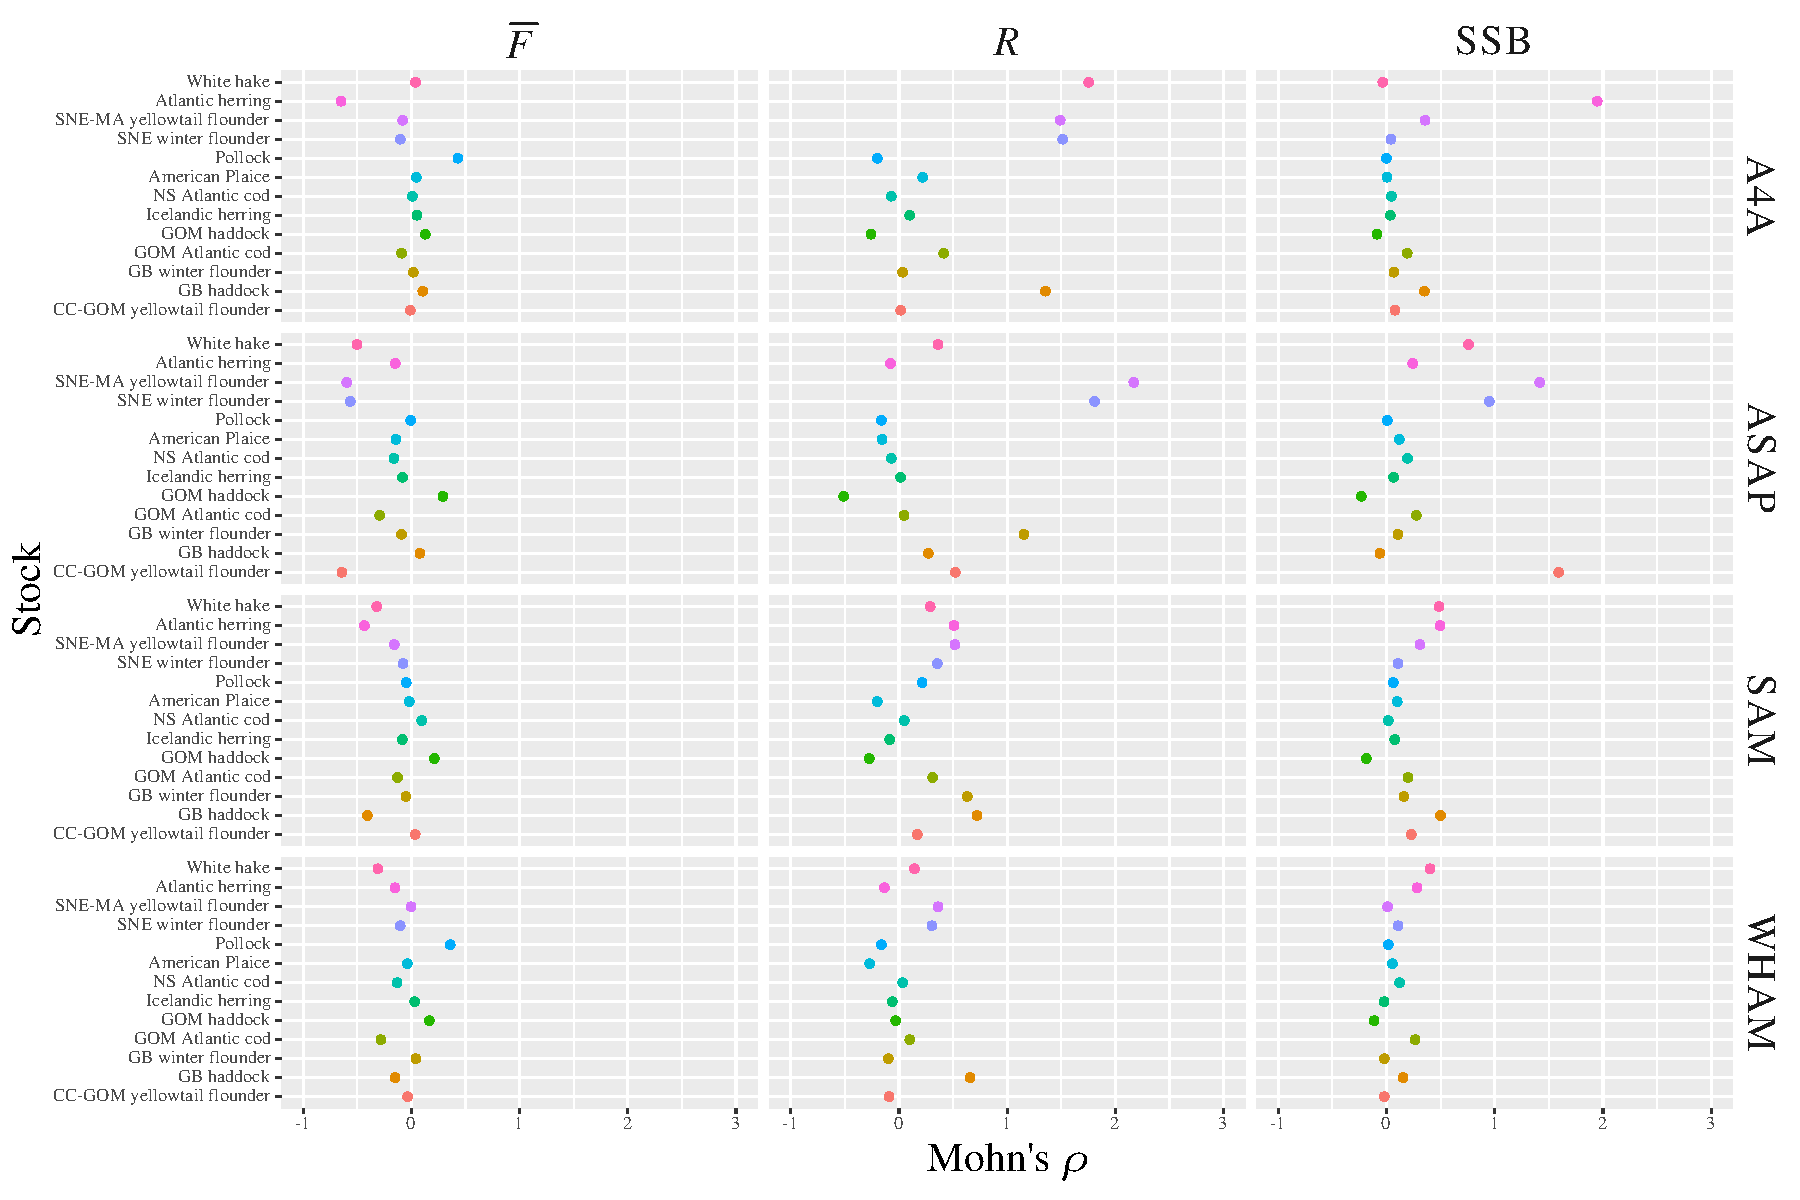
\includegraphics[height = 0.9\textheight]{../db/rho_paper_plot.pdf}
\end{center}
\end{figure}

%\begin{figure}
%\caption{Relationship between Mohn's $\rho$ for SSB and average fishing mortality by model.}\label{rho_ssb_vs_F}
%\begin{center}
%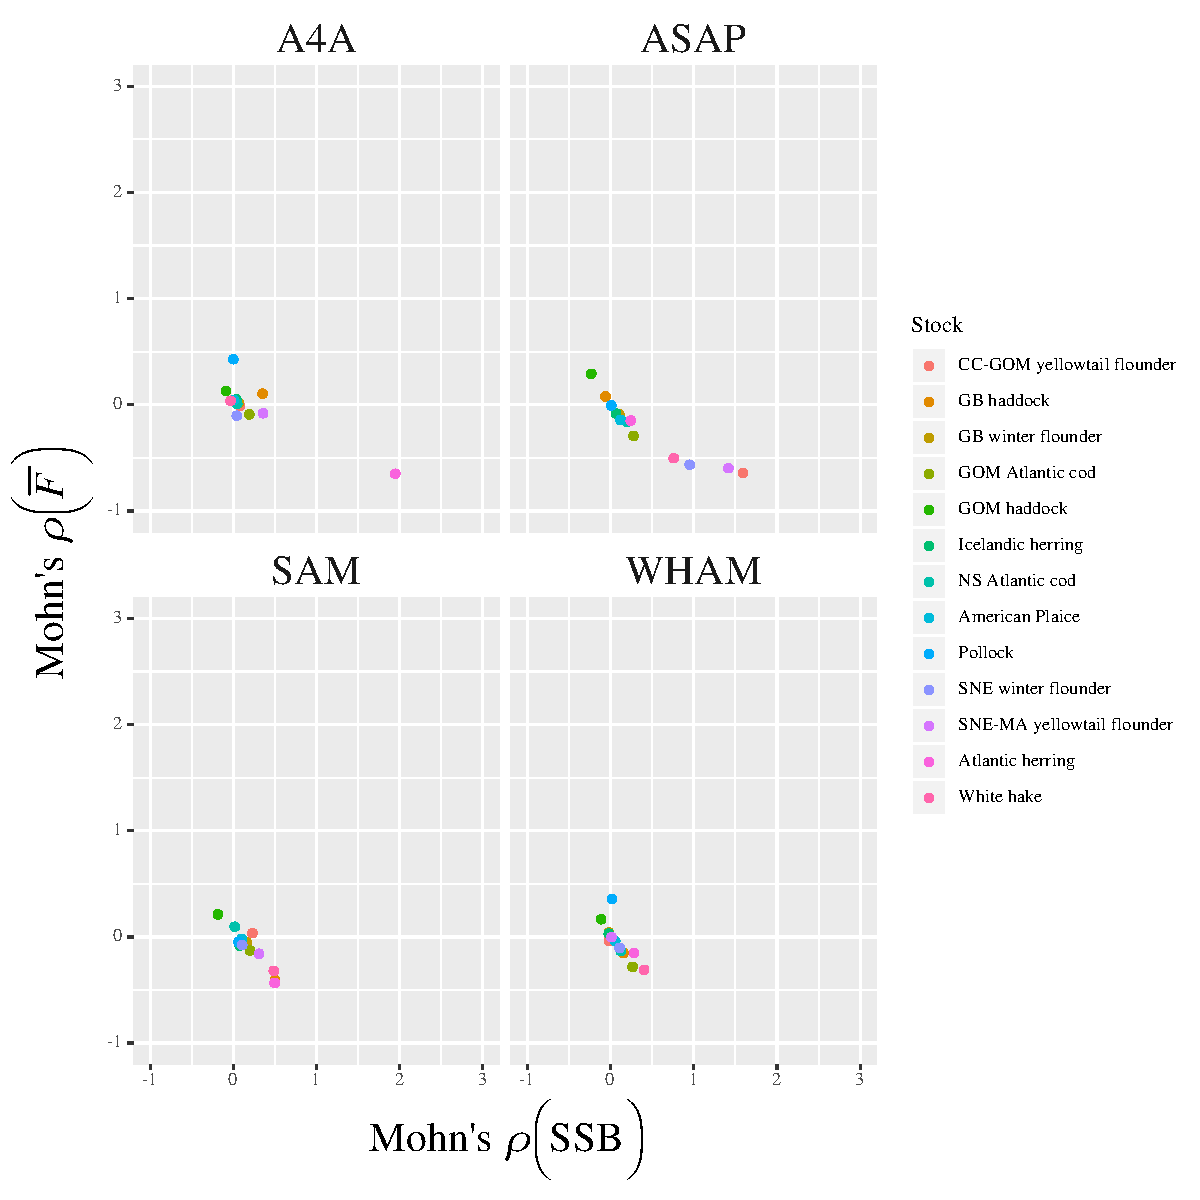
\includegraphics[height = 0.9\textheight]{../db/SSBvsFbarMohnRho_paper.pdf}
%\end{center}
%\end{figure}

\begin{figure}
\caption{Bias of predicted indices at age in the final 3 years of the model that were presumed missing in model fits.}\label{predmissing_biasplot}
\begin{center}
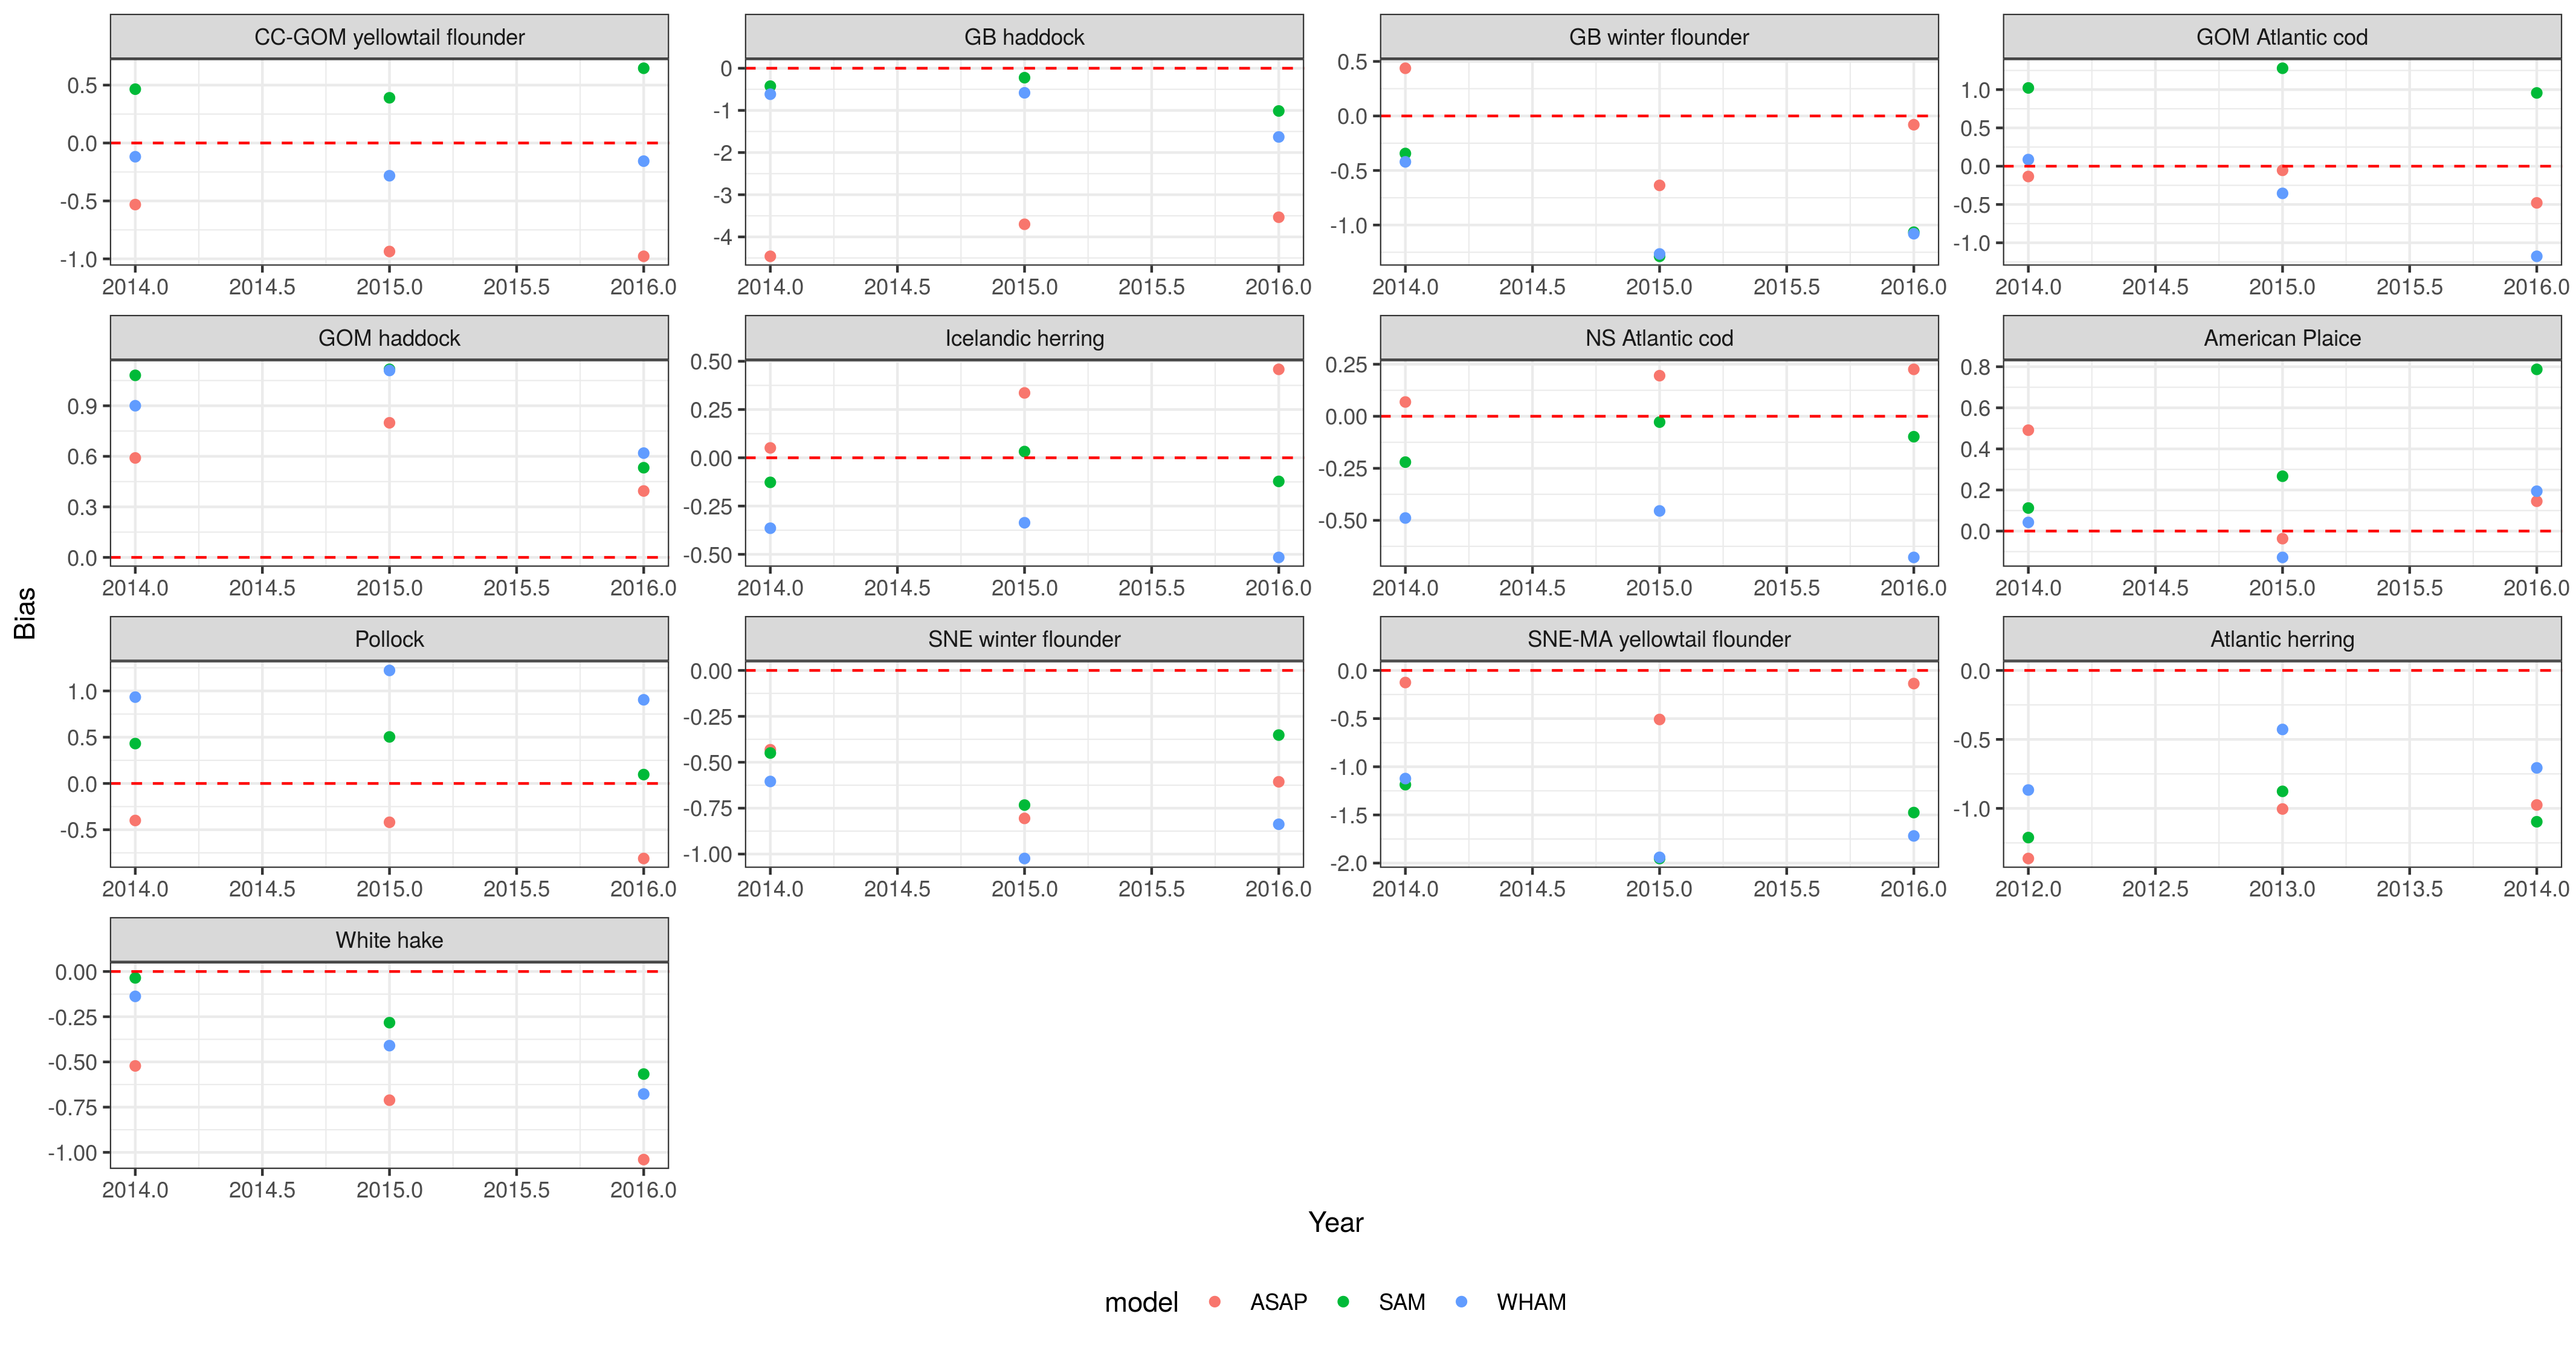
\includegraphics[height = 0.8\textheight]{../db/predmissing_biasplot.png}
\end{center}
\end{figure}

\begin{figure}
\caption{Root mean square error of predicted indices at age in the final 3 years of the model that were presumed missing in model fits.}\label{predmissing_rmseplot}
\begin{center}
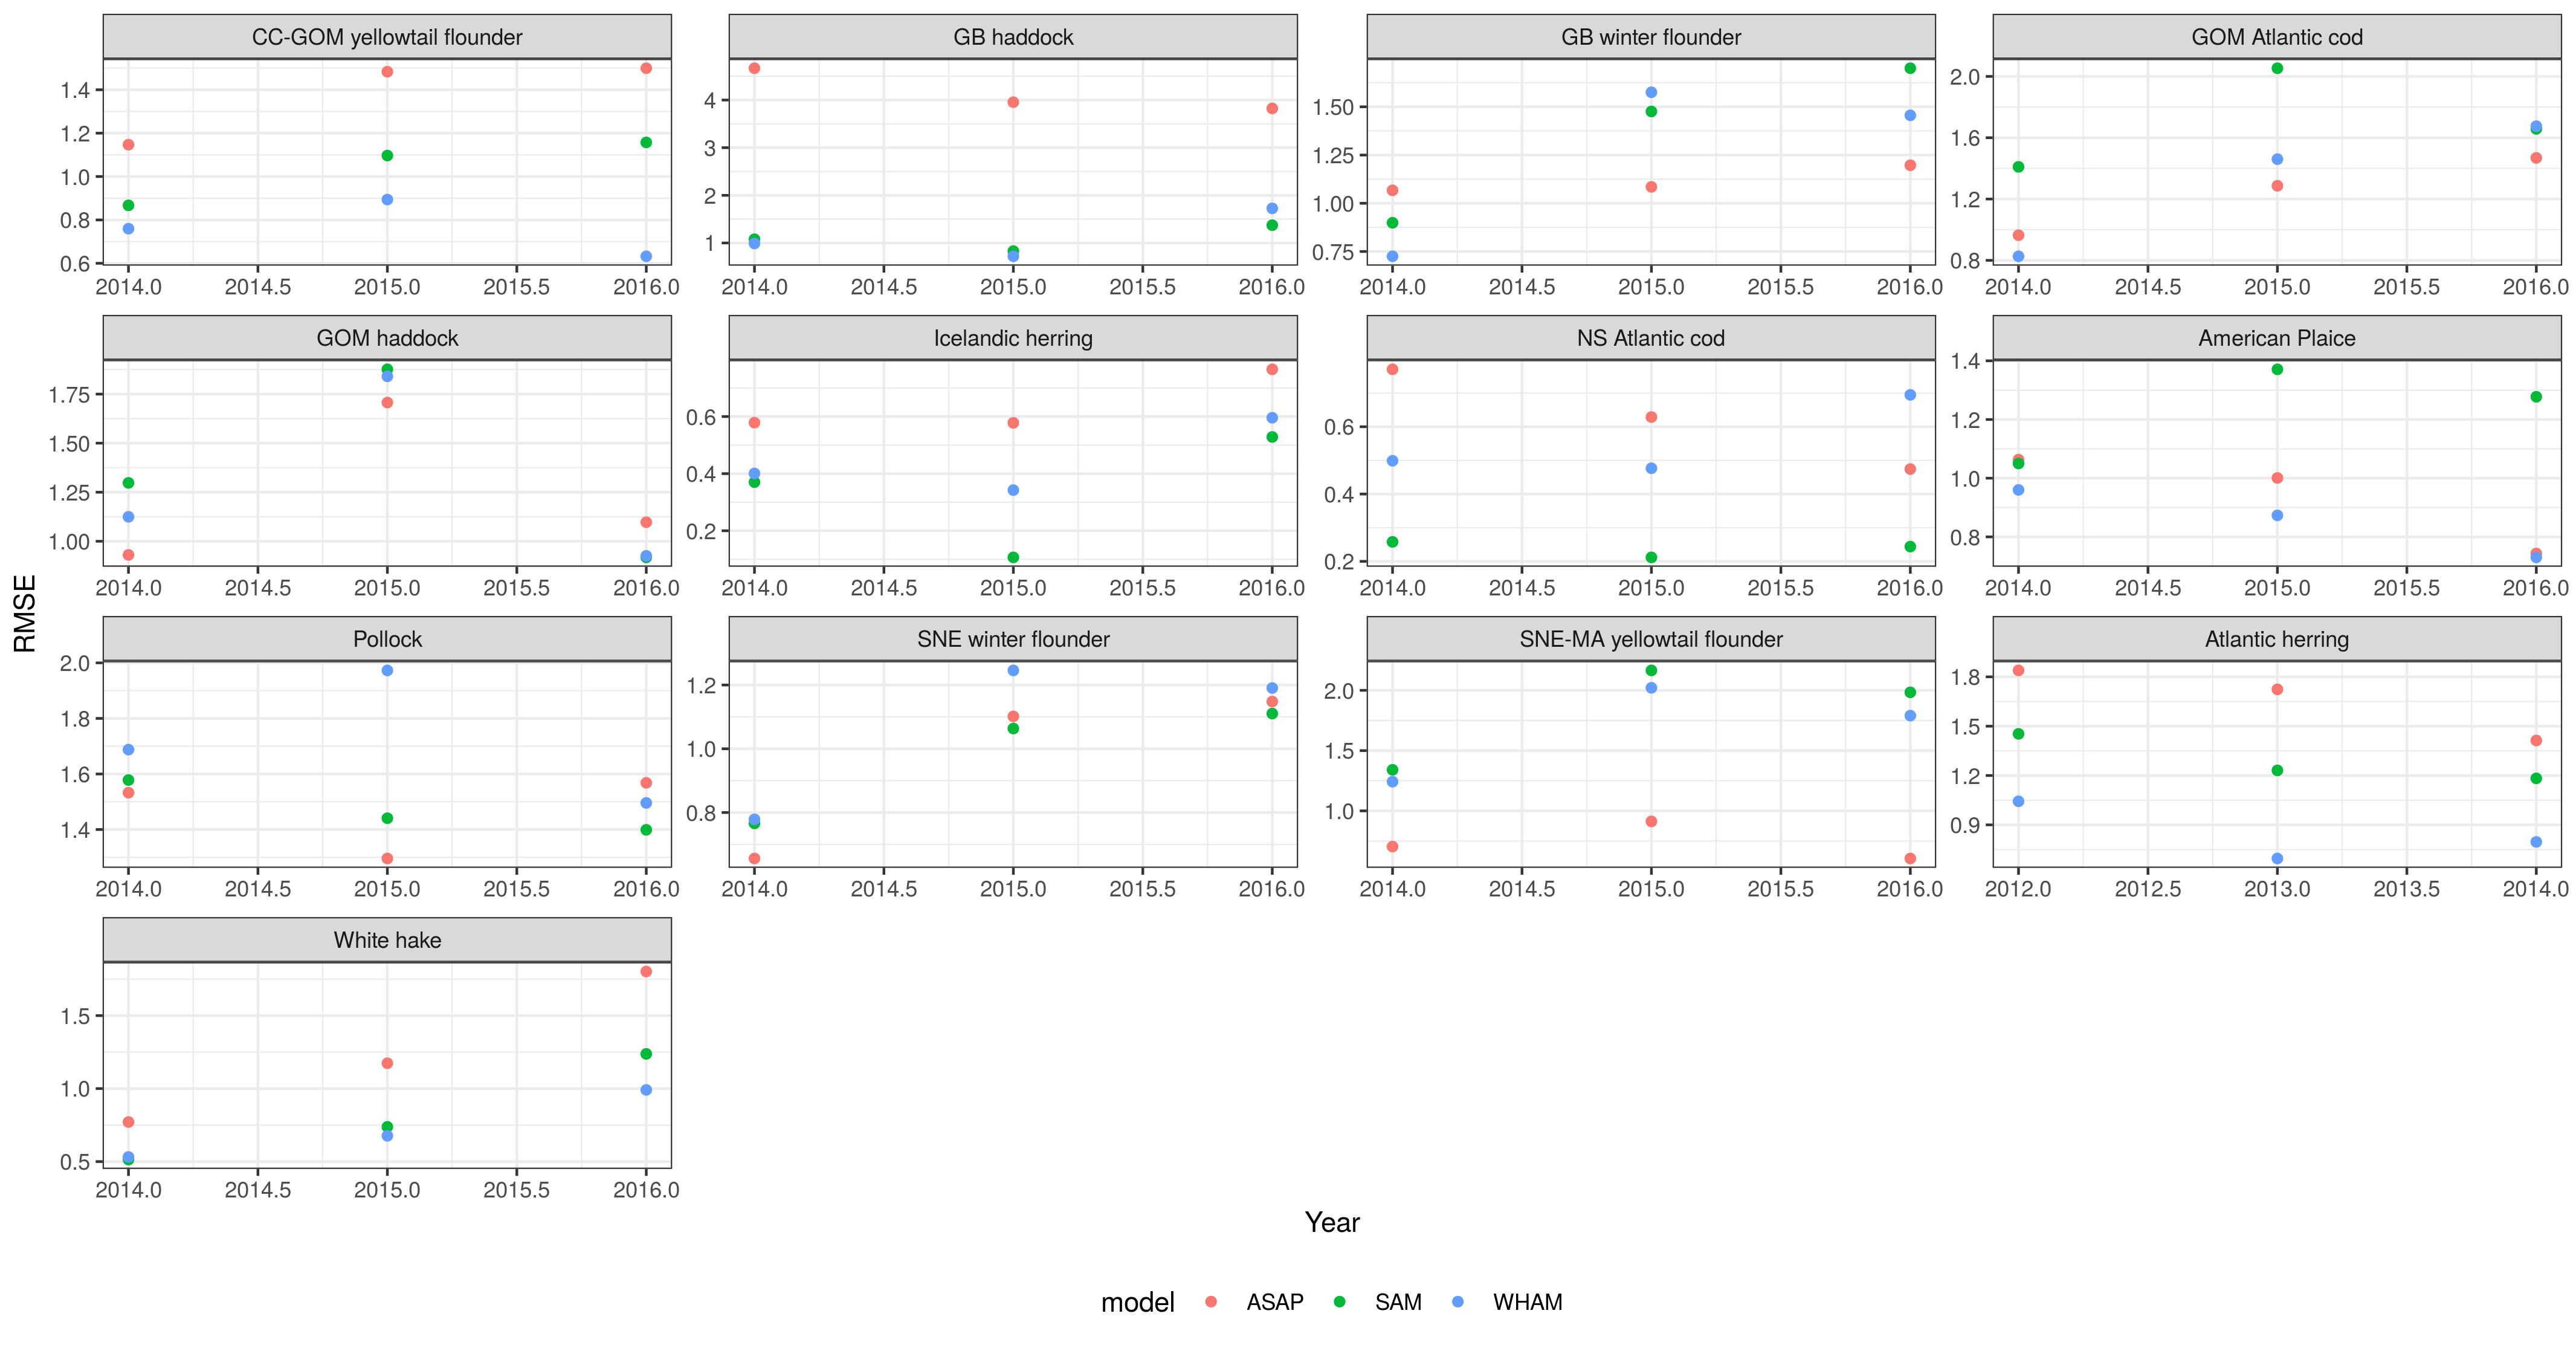
\includegraphics[height = 0.8\textheight]{../db/predmissing_rmseplot.png}
\end{center}
\end{figure}

\begin{figure}
\caption{Average bias of predicted indices at age in the final 3 years of the model that were presumed missing in model fits across all 13 stocks.}\label{predmissing_avgbiasplot}
\begin{center}
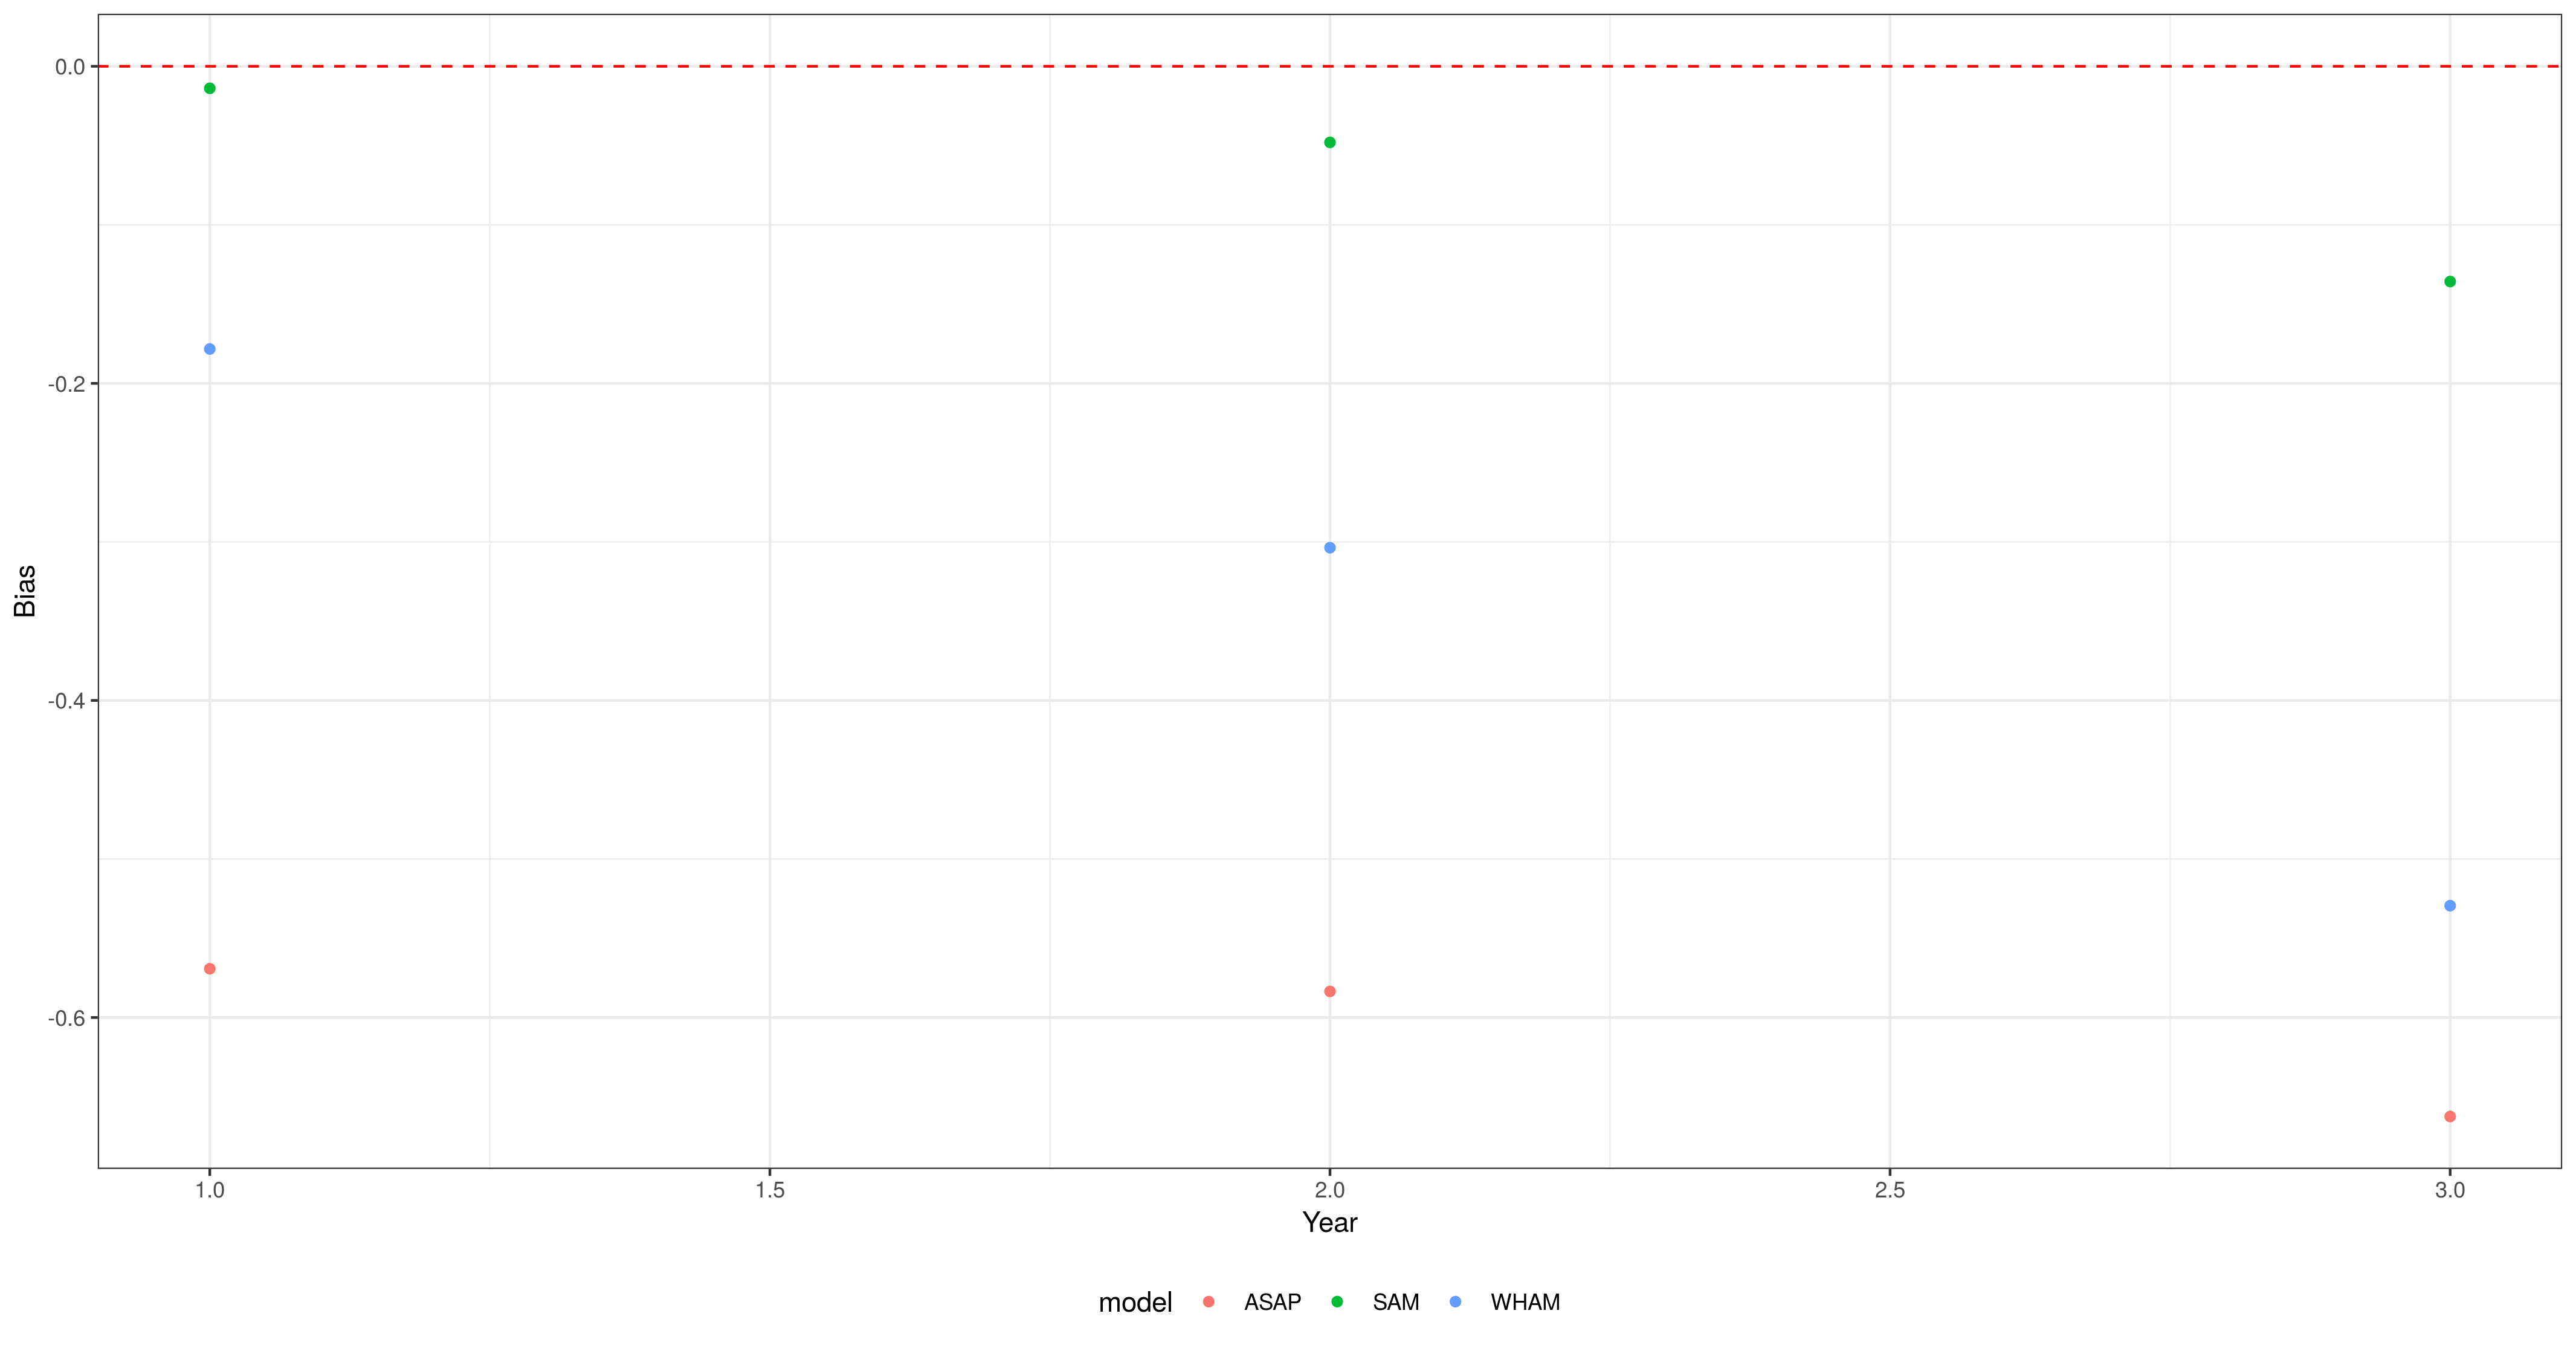
\includegraphics[height = 0.8\textheight]{../db/predmissing_avgbiasplot.png}
\end{center}
\end{figure}


\begin{figure}
\caption{Average root mean square error of predicted indices at age in the final 3 years of the model that were presumed missing in model fits across all 13 stocks.}\label{predmissing_avgrmseplot}
\begin{center}
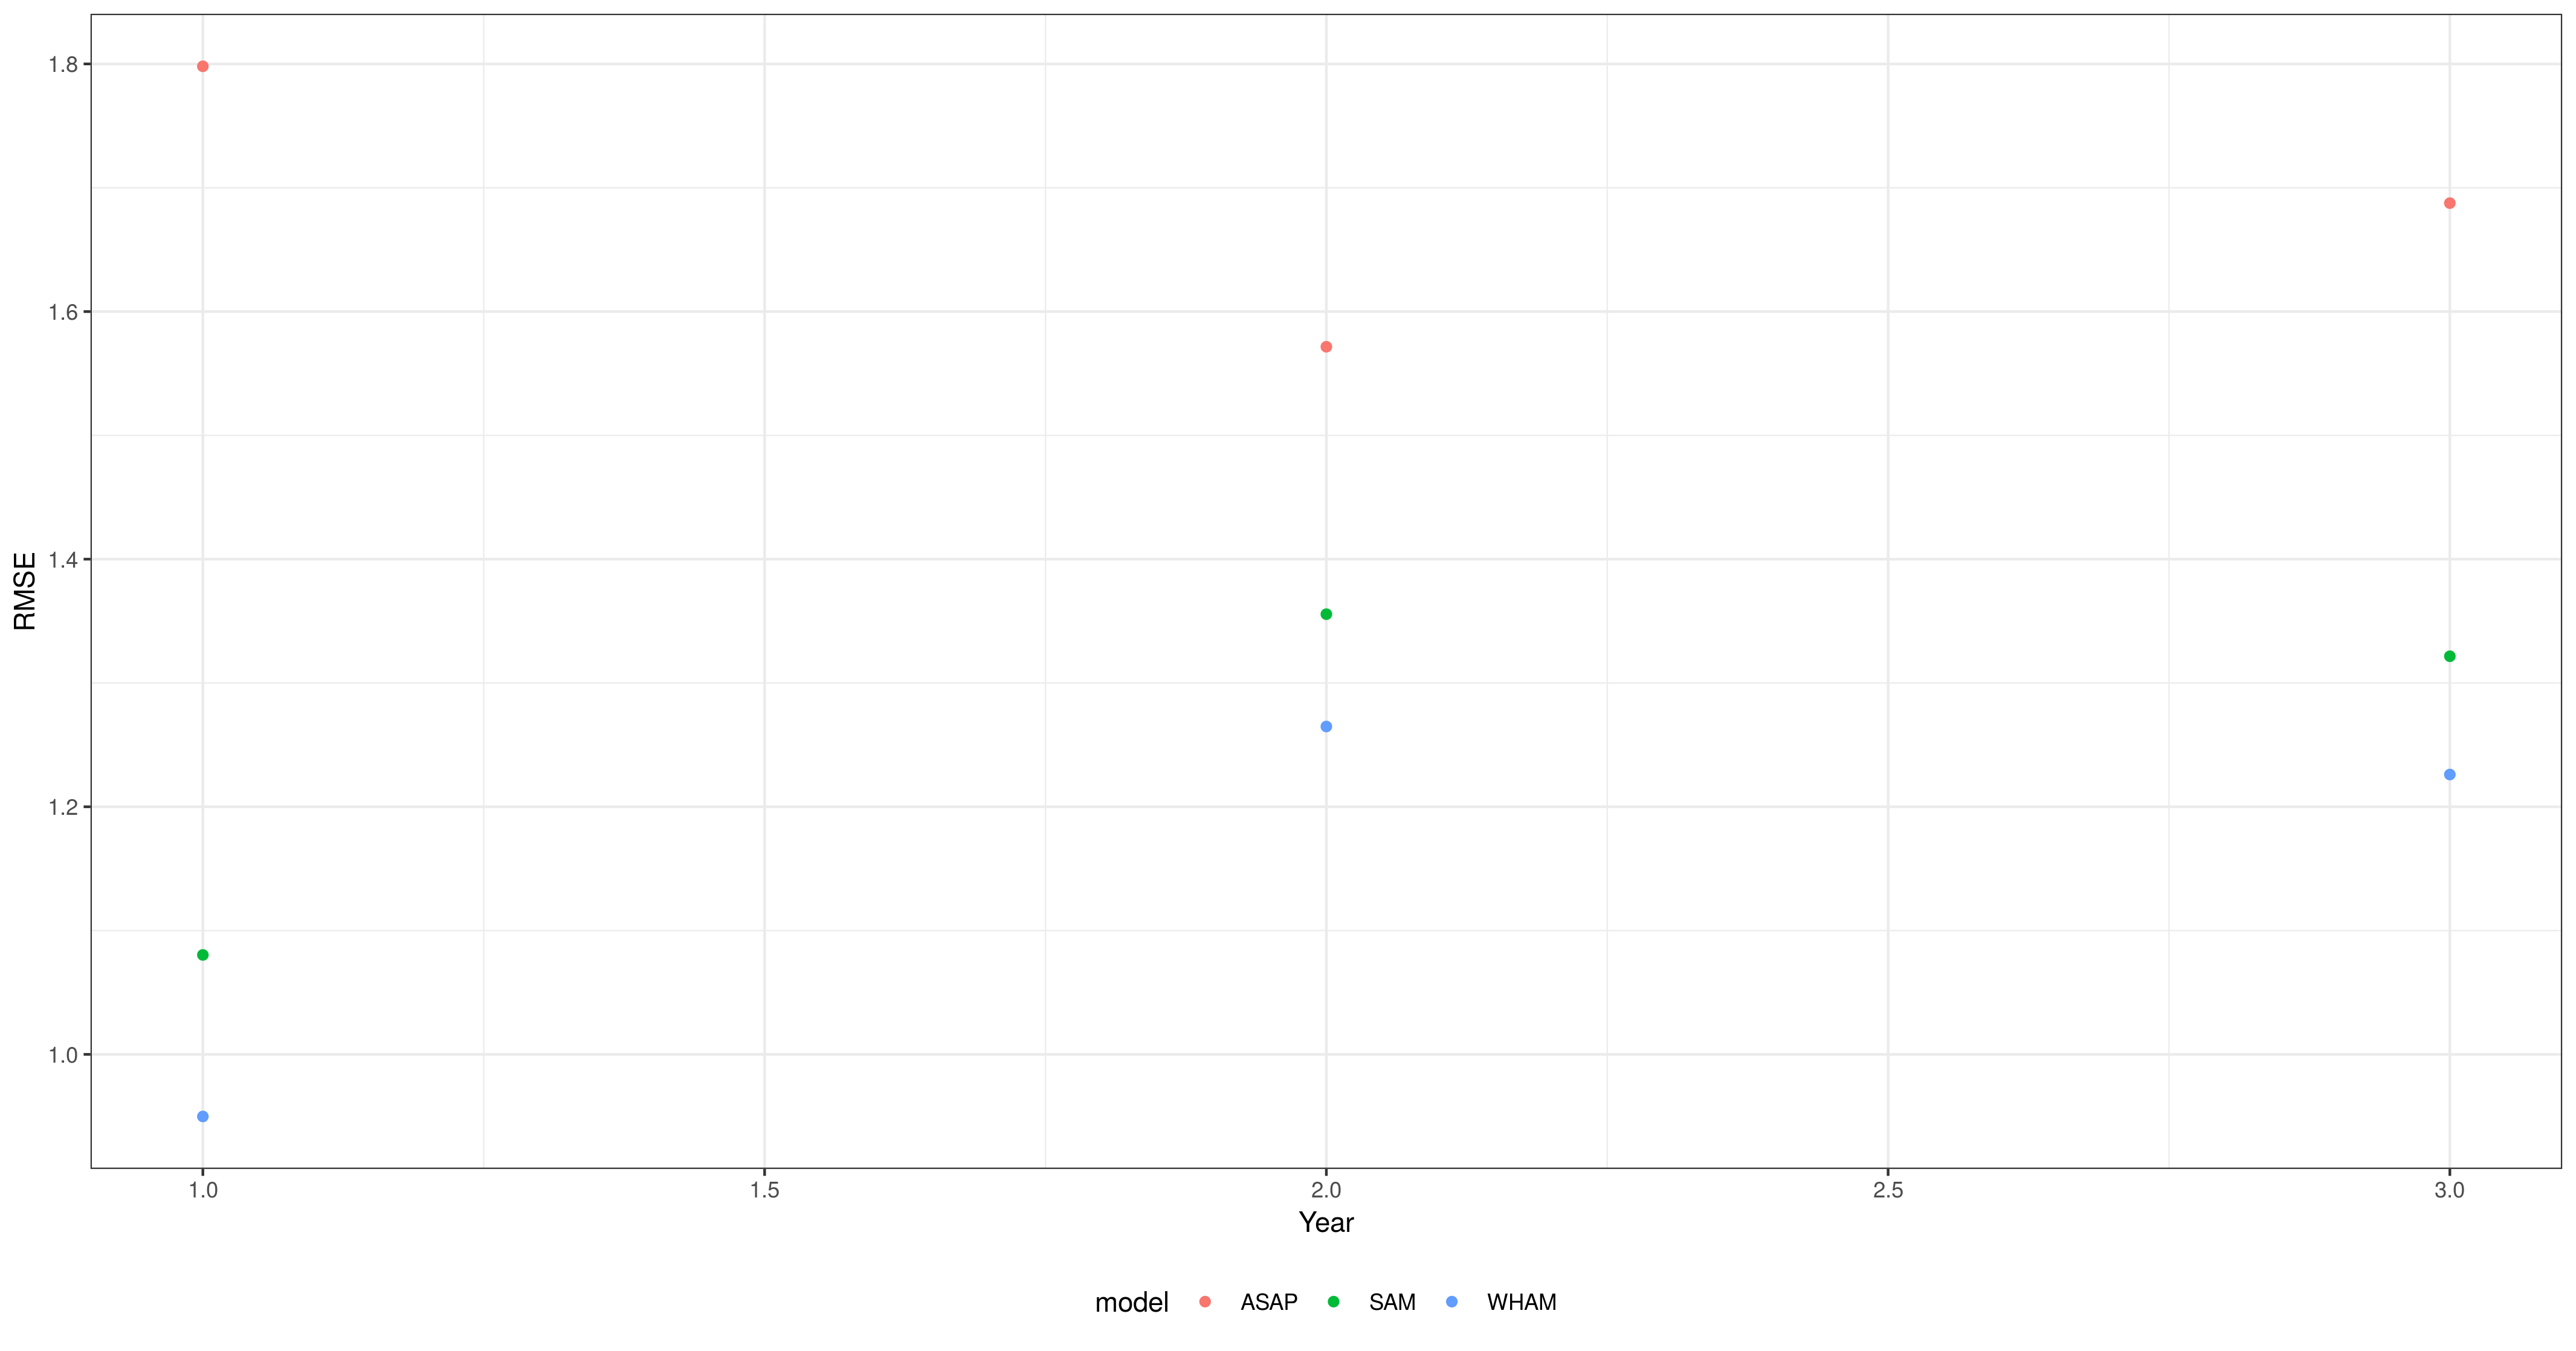
\includegraphics[height = 0.8\textheight]{../db/predmissing_avgrmseplot.png}
\end{center}
\end{figure}

\begin{figure}
\caption{Average root mean square error of predicted indices at age in the final 3 years of the model that were presumed missing in model fits across all 13 stocks.}\label{predmissing_avgrmseplot}
\begin{center}
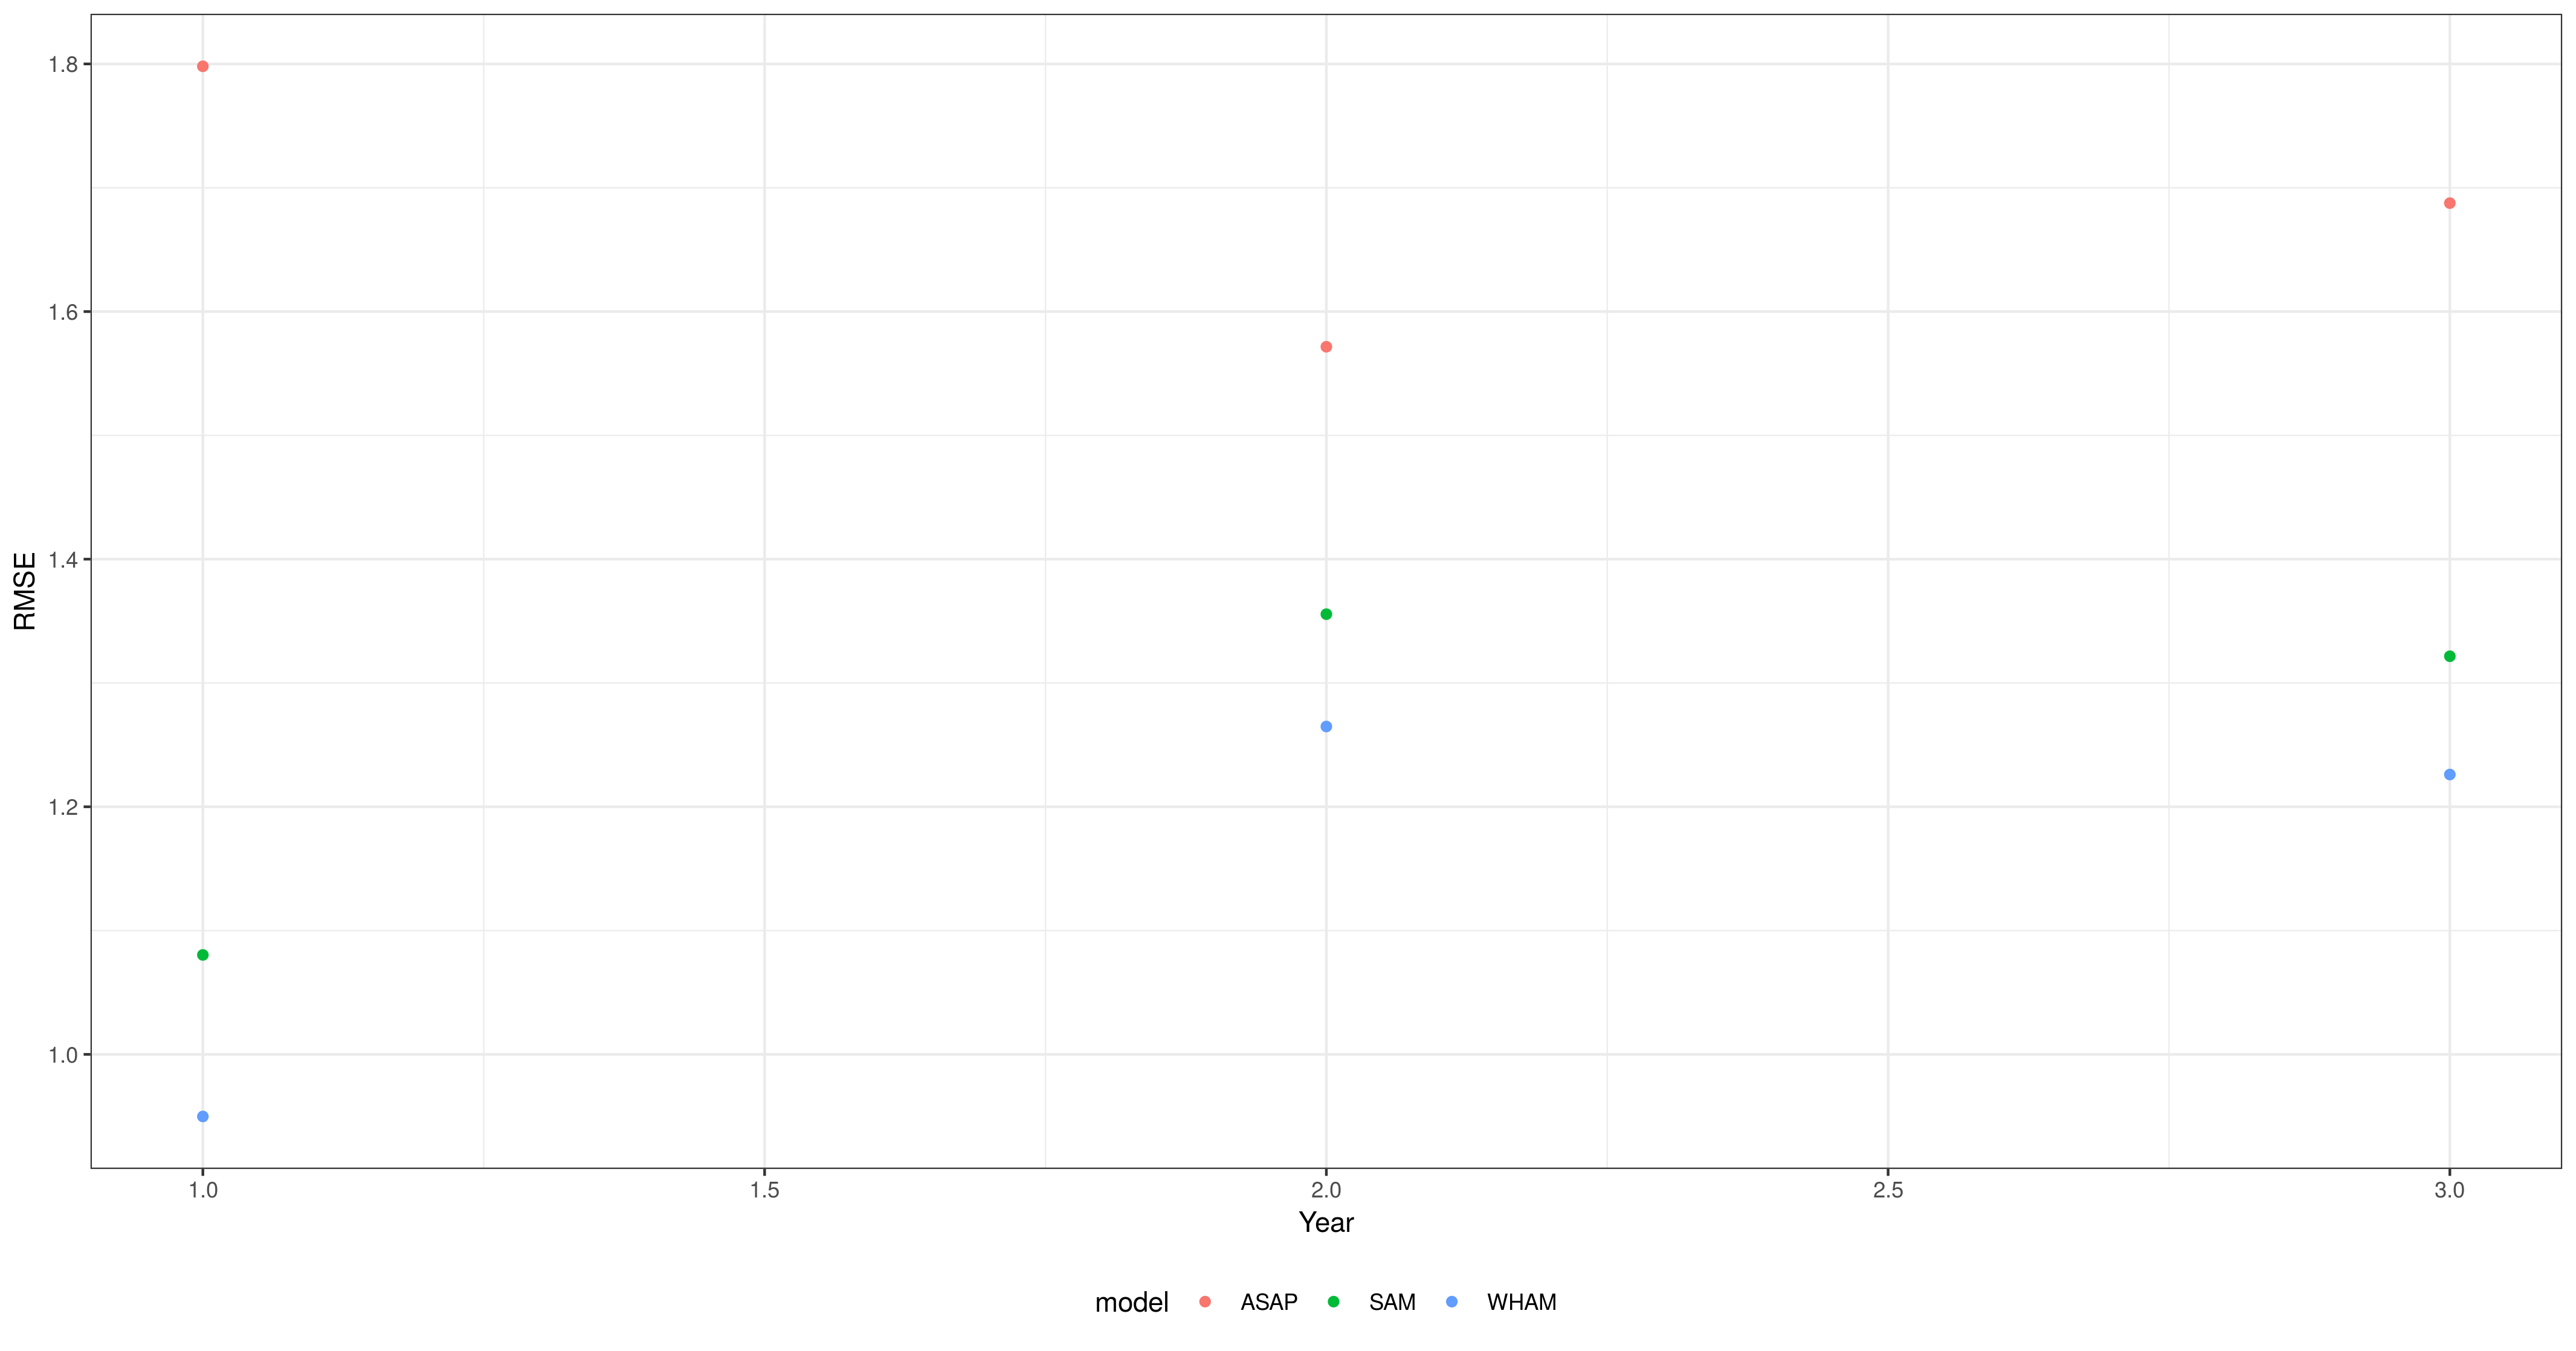
\includegraphics[height = 0.8\textheight]{../db/predmissing_avgrmseplot.png}
\end{center}
\end{figure}

%WHAM plots
\begin{figure}
\caption{Degree of retrospective pattern in average fishing mortality, recruitment, and spawning stock biomass as measured by Mohn's $\rho$ for each stock and WHAM model configuration.}\label{wham_rho_paper_plot}
\begin{center}
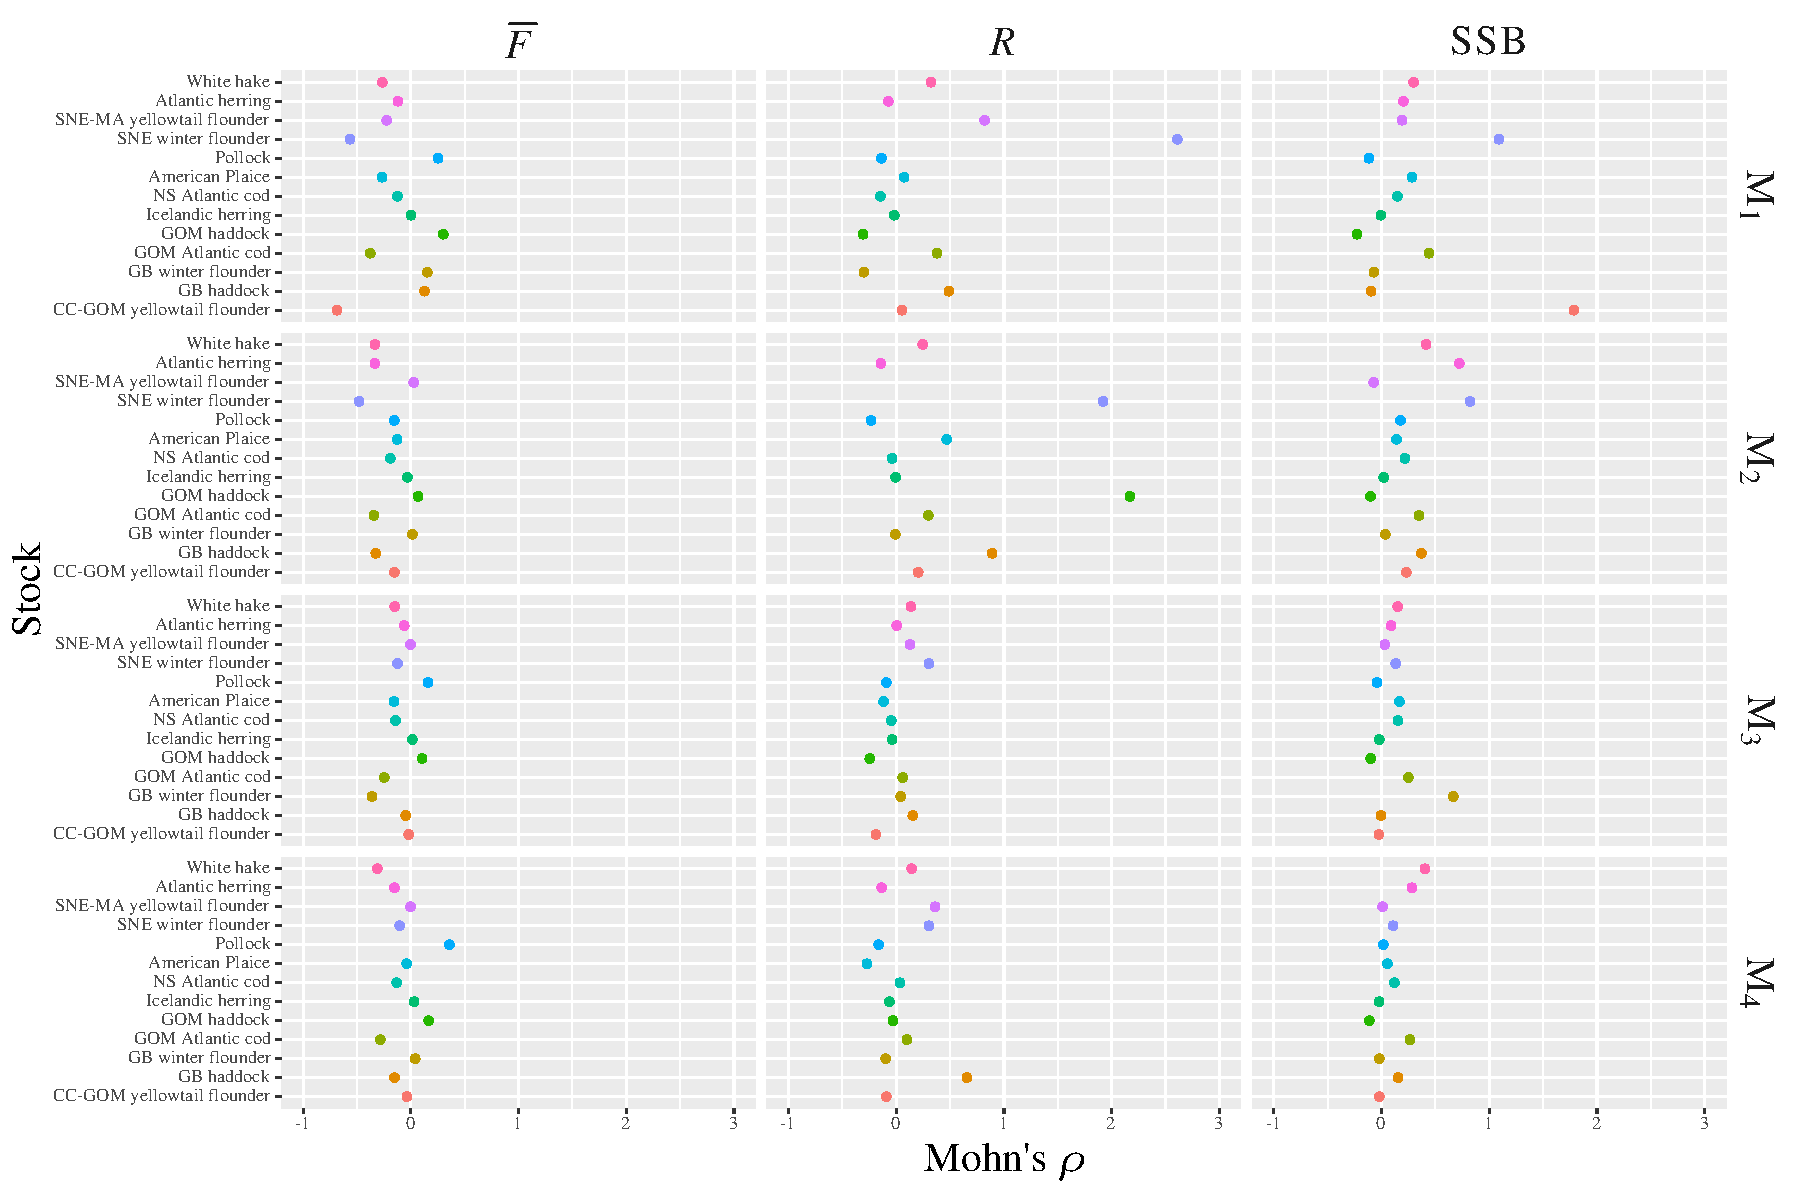
\includegraphics[height = 0.9\textheight]{../db/wham_rho_paper_plot.pdf}
\end{center}
\end{figure}

\begin{figure}
\caption{Estimated coefficient of variation for annual spawning stock biomass estimates for each stock and WHAM model configuration.}\label{wham_SSB_CV}
\begin{center}
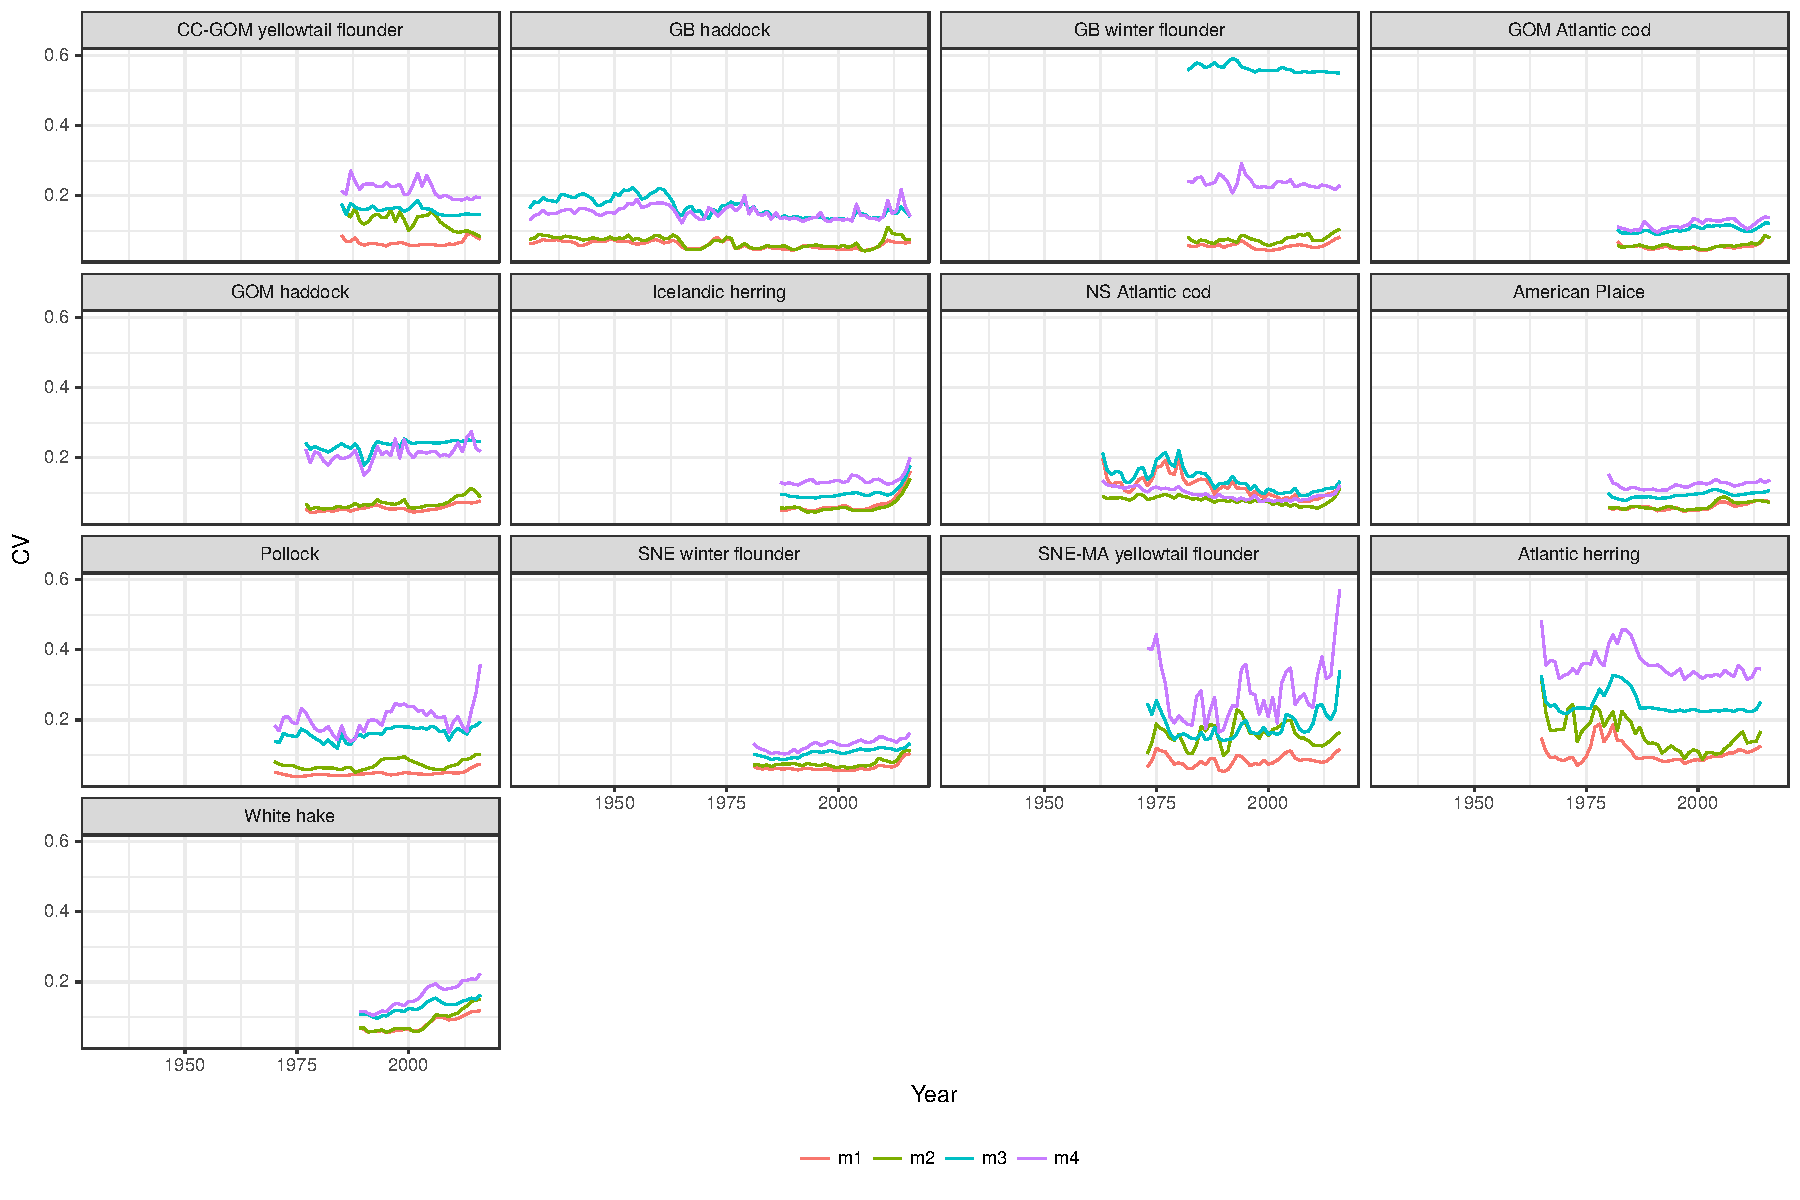
\includegraphics[height = 0.9\textheight]{wham_SSB_CV.pdf}
\end{center}
\end{figure}

\begin{figure}
\caption{Ratio of estimated coefficient of variation for annual spawning stock biomass estimates using state-space and SCAA models with a given distributional assumption for age composition observations.}\label{wham_SSB_CV_ratio}
\begin{center}
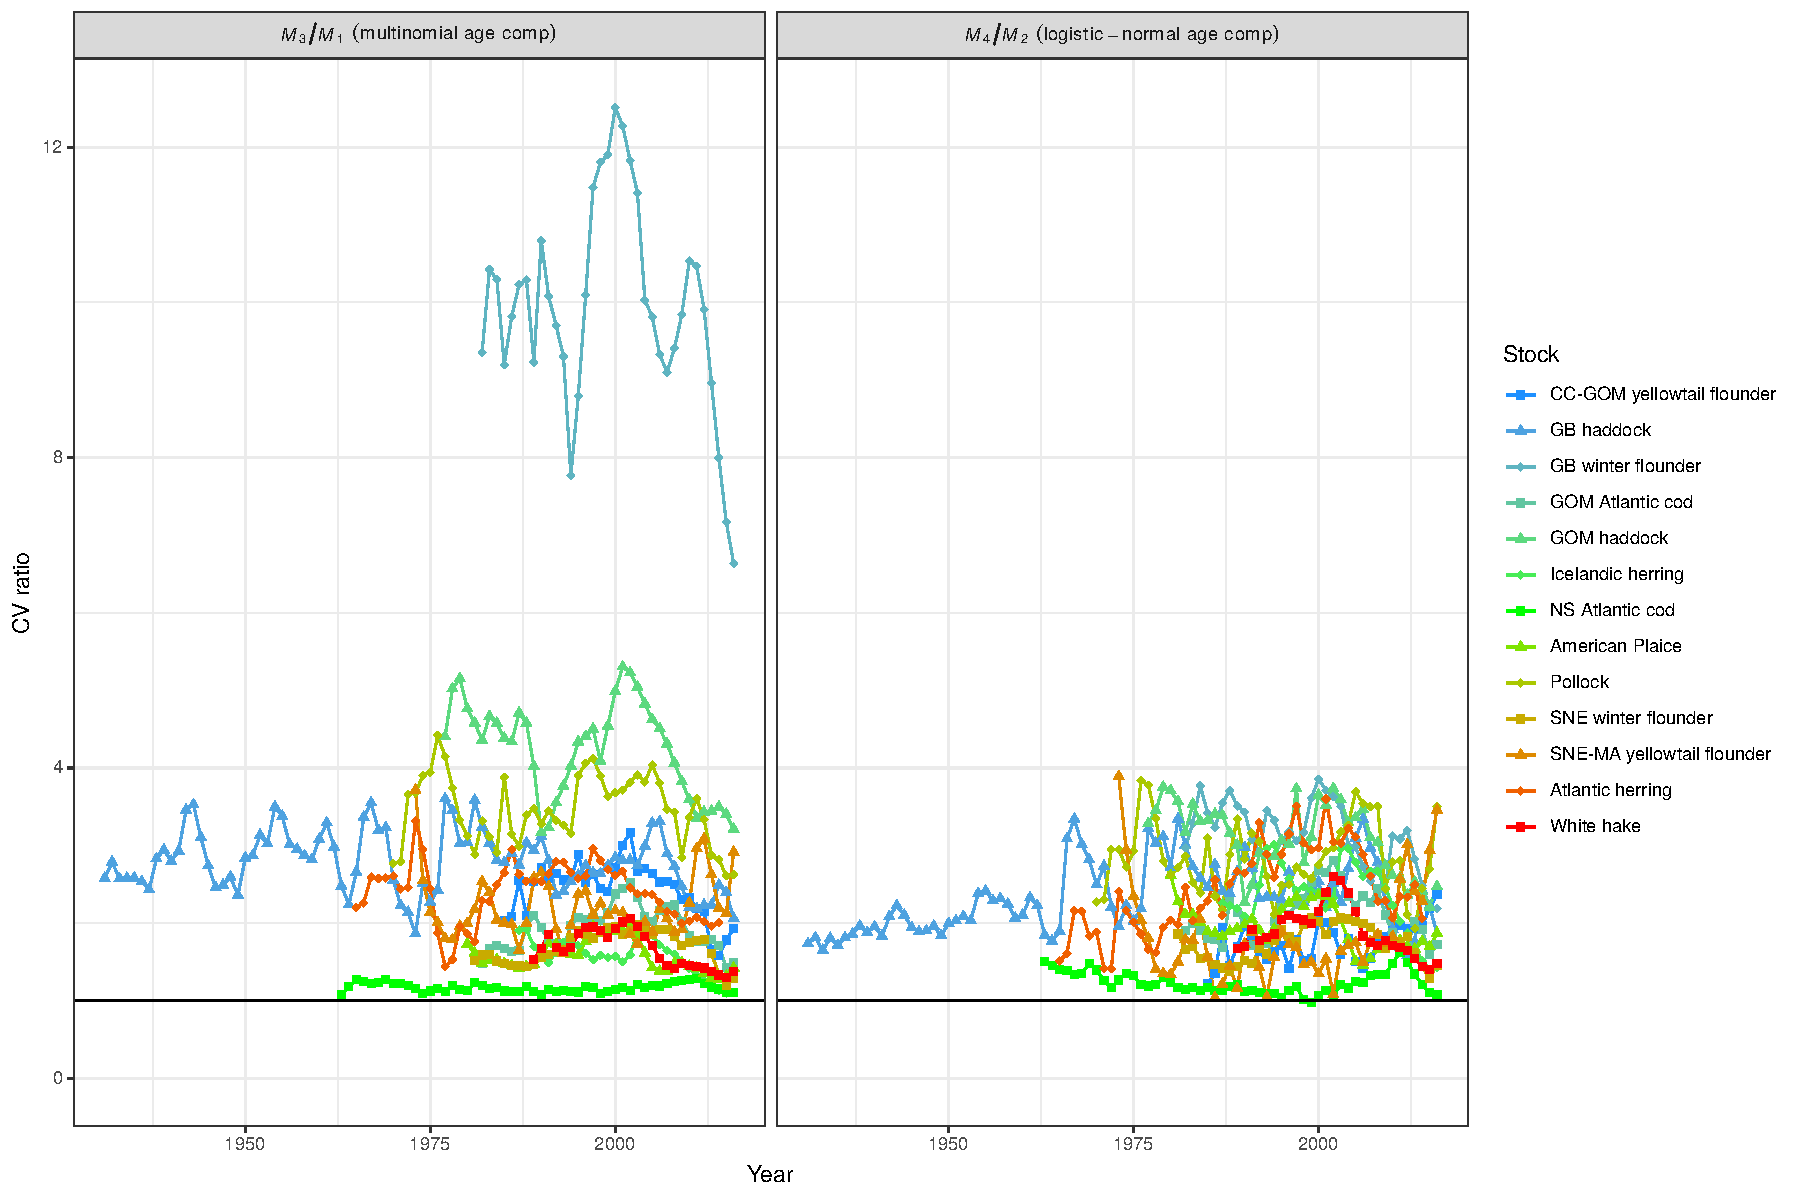
\includegraphics[height = 0.9\textheight]{wham_CV_ratio_SSB.pdf}
\end{center}
\end{figure}
\end{landscape}

\clearpage

%Tables

\begin{landscape}
\begin{table}
\begin{center}
\caption{Modelling assumptions for the four estimation models.}\label{assumption_models}

\begin{tabular}{lllll}
\toprule
Assumptions & A4A & ASAP & WHAM & SAM\\
\midrule
Total catch & ? & Log-normal & Log-normal & NA\\
Catch age composition & ? & Multinomial & Multinomial & NA\\ 
Catch at age & ? & NA & NA & Log-normal\\
Fit to total survey index & & Log-normal & Log-normal & NA\\
Fit to survey index age composition & & Multinomial & Multinomial & NA \\
Fit to survey index at age matrix & & NA & NA & Log-normal\\
Recruitment & & & Log-normal iid random effect & Log-normal iid random effect\\
Max annual fishing mortality & Fixed effect & Fixed effects & Fixed effects & NA\\
Fishing mortality at age & Smoother & NA & NA & Log-normal random walk\\
Transitions in numbers at age & Deterministic & Deterministic & Log-normal random effect & Log-normal random effect \\
Comments & & & & \\
\bottomrule
\end{tabular}

\end{center}
\end{table}

\begin{table}
\begin{center}
\caption{Fish stocks considered in this study.}\label{fish_stocks}
% Possibility of reducing name code and use the same in figures so legend/labels less long
\begin{tabular}{lllll}
\toprule
Fish stock & Name code & Current Model & No. Surveys & Reference\\
\midrule
Cape Cod-Gulf of Maine yellowtail flounder & CC-GOM yellowtail flounder & VPA & 4 & \citet{nefsc17} \\
Georges Bank haddock & GB haddock & VPA & 3 & \citet{nefsc17} \\
Georges Bank winter flounder & GB winter flounder & VPA & 3 & \citet{nefsc17} \\
Gulf of Maine Atlantic cod & GOM Atlantic cod & ASAP & 3 & \citet{nefsc17} \\
Gulf of Maine haddock & GOM haddock & ASAP & 2 & \citet{nefsc17} \\
Icelandic herring & Icelandic herring & VPA & 1 & \\
North Sea Atlantic cod & NS cod & SAM & 2 & \citet{ices18}\\
American plaice & American plaice & VPA & 4 & \citet{nefsc17} \\
Pollock & Pollock & ASAP & 2 & \citet{nefsc17} \\
Southern New England-Mid Atlantic winter flounder & SNE winter flounder & ASAP & 3 & \citet{nefsc17} \\
Southern New England-Mid Atlantic yellowtail flounder & SNE-MA yellowtail flounder & ASAP & 2 & \citet{nefsc17} \\
US Atlantic herring & Atlantic herring & ASAP & 2 & \citet{deroba15} \\
White hake & White hake & ASAP & 2 & \citet{nefsc17} \\
\bottomrule
\end{tabular}

\end{center}
\end{table}

\end{landscape}

\begin{table}
\begin{center}
\caption{Mean and Standard Deviation of Mohn's $\rho$ for SSB, $\overline{F}$, and recruitment across all stocks by model type.}\label{model_compare}

\begin{tabular}{lrr}
\toprule
Model & Mean & SD\\
\midrule
\addlinespace[0.3em]
\multicolumn{3}{l}{$\overline{F}$}\\
\hspace{1em}A4A & -0.01 & 0.24\\
\hspace{1em}ASAP & -0.22 & 0.28\\
\hspace{1em}SAM & -0.11 & 0.19\\
\hspace{1em}WHAM & -0.05 & 0.18\\
\addlinespace[0.3em]
\multicolumn{3}{l}{$R$}\\
\hspace{1em}A4A & 1.13 & 2.30\\
\hspace{1em}ASAP & 0.41 & 0.81\\
\hspace{1em}SAM & 0.25 & 0.31\\
\hspace{1em}WHAM & 0.06 & 0.26\\
\addlinespace[0.3em]
\multicolumn{3}{l}{SSB}\\
\hspace{1em}A4A & 0.23 & 0.53\\
\hspace{1em}ASAP & 0.42 & 0.58\\
\hspace{1em}SAM & 0.20 & 0.21\\
\hspace{1em}WHAM & 0.09 & 0.15\\
\bottomrule
\end{tabular}

\end{center}
\end{table}

\end{document}
